\fancyhead[LH]{复旦大学软件工程}
\fancyhead[RH]{第五章\quad 静态建模}
\section{静态建模}






\subsection{类图}
\subsubsection{信息管理系统类图}
\begin{figure}[H] 
    \center{
\includegraphics[scale=0.56]{OOA/fig/1-信息管理/I-类图.pdf}} 
    \bicaption{Volunet信息管理系统类图}{Class Diagram for Information Management System of Volunet} 
\end{figure}

\subsubsection{志愿服务系统类图}
\begin{figure}[H] 
    \center{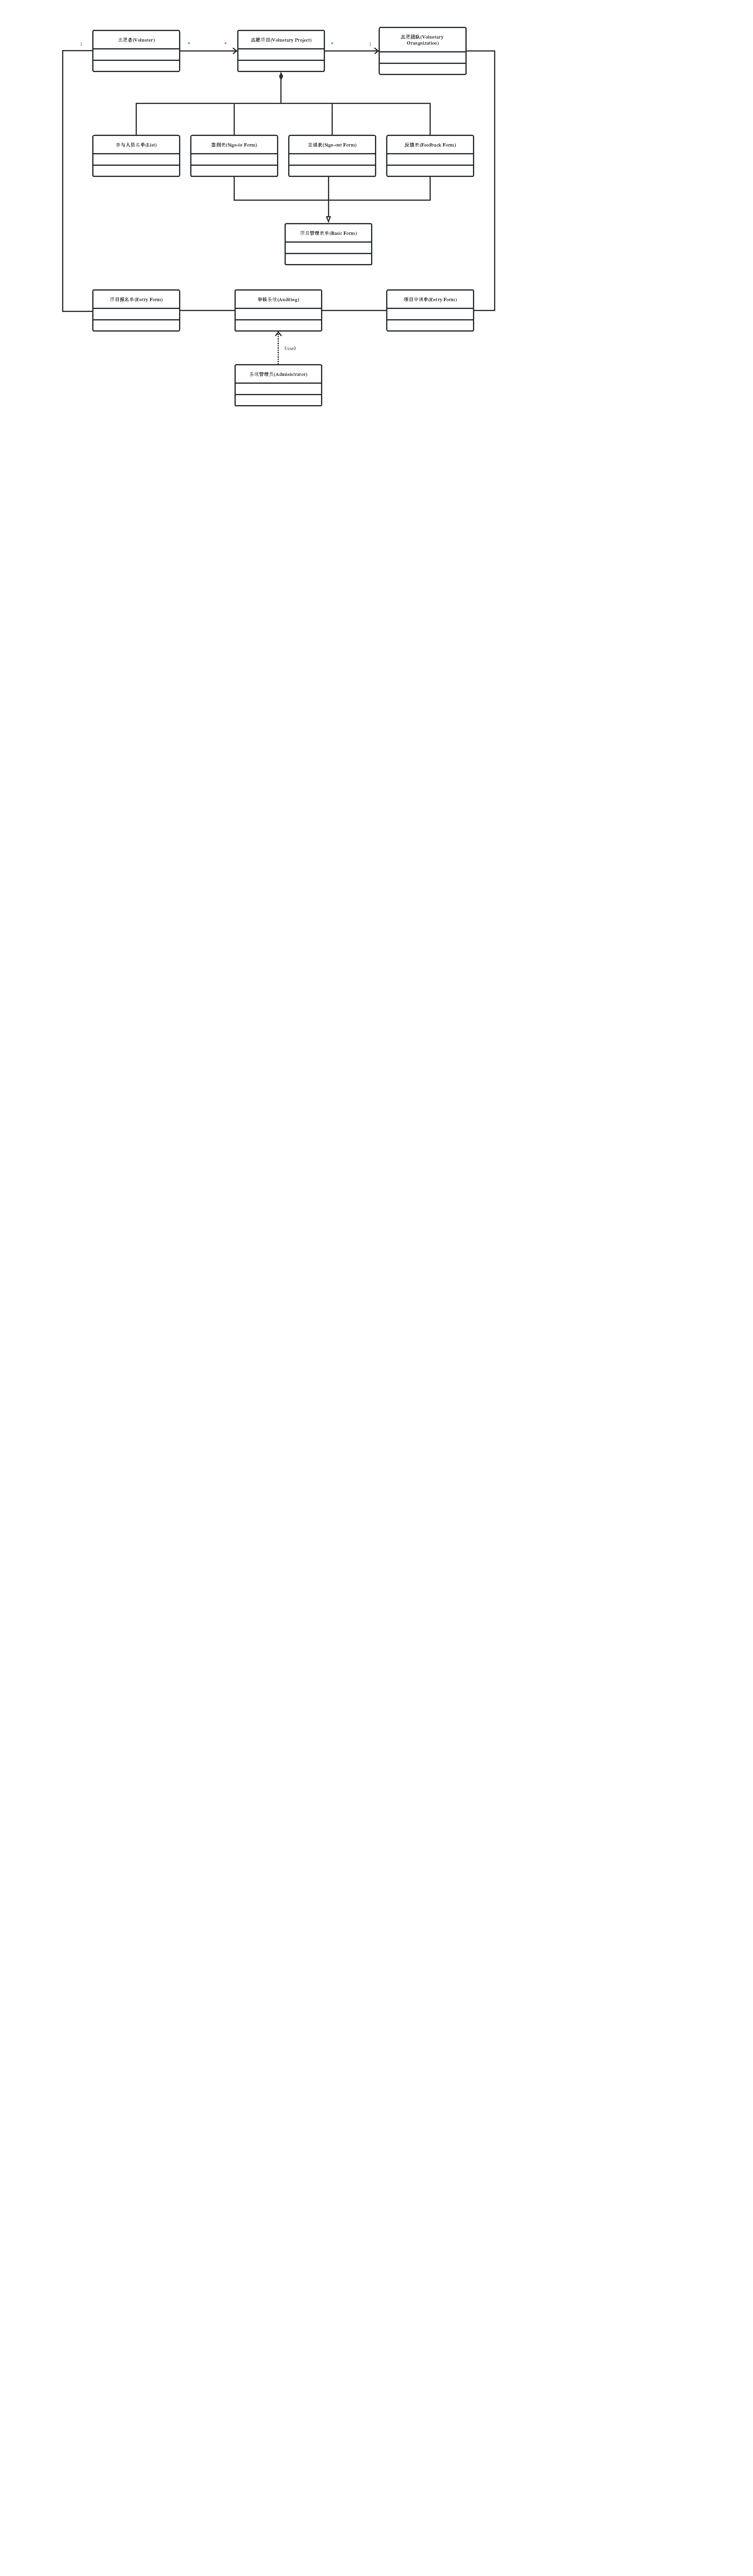
\includegraphics[scale=0.56]{OOA/fig/2-志愿服务/VS-类图.pdf}} 
    \bicaption{Volunet志愿服务系统类图}{Class Diagram for Voluntary Service System of Volunet} 
\end{figure}

\subsubsection{爱心捐助系统类图}
\begin{figure}[H] 
    \center{\includegraphics[scale=0.35]{OOA/fig/3-爱心管理/爱心管理类图-1.pdf}} 
    \bicaption{Volunet爱心捐助系统类图}{Class Diagram for Love Donation System of Volunet} 
\end{figure}

\subsubsection{公益课程系统类图}
\begin{figure}[H] 
    \center{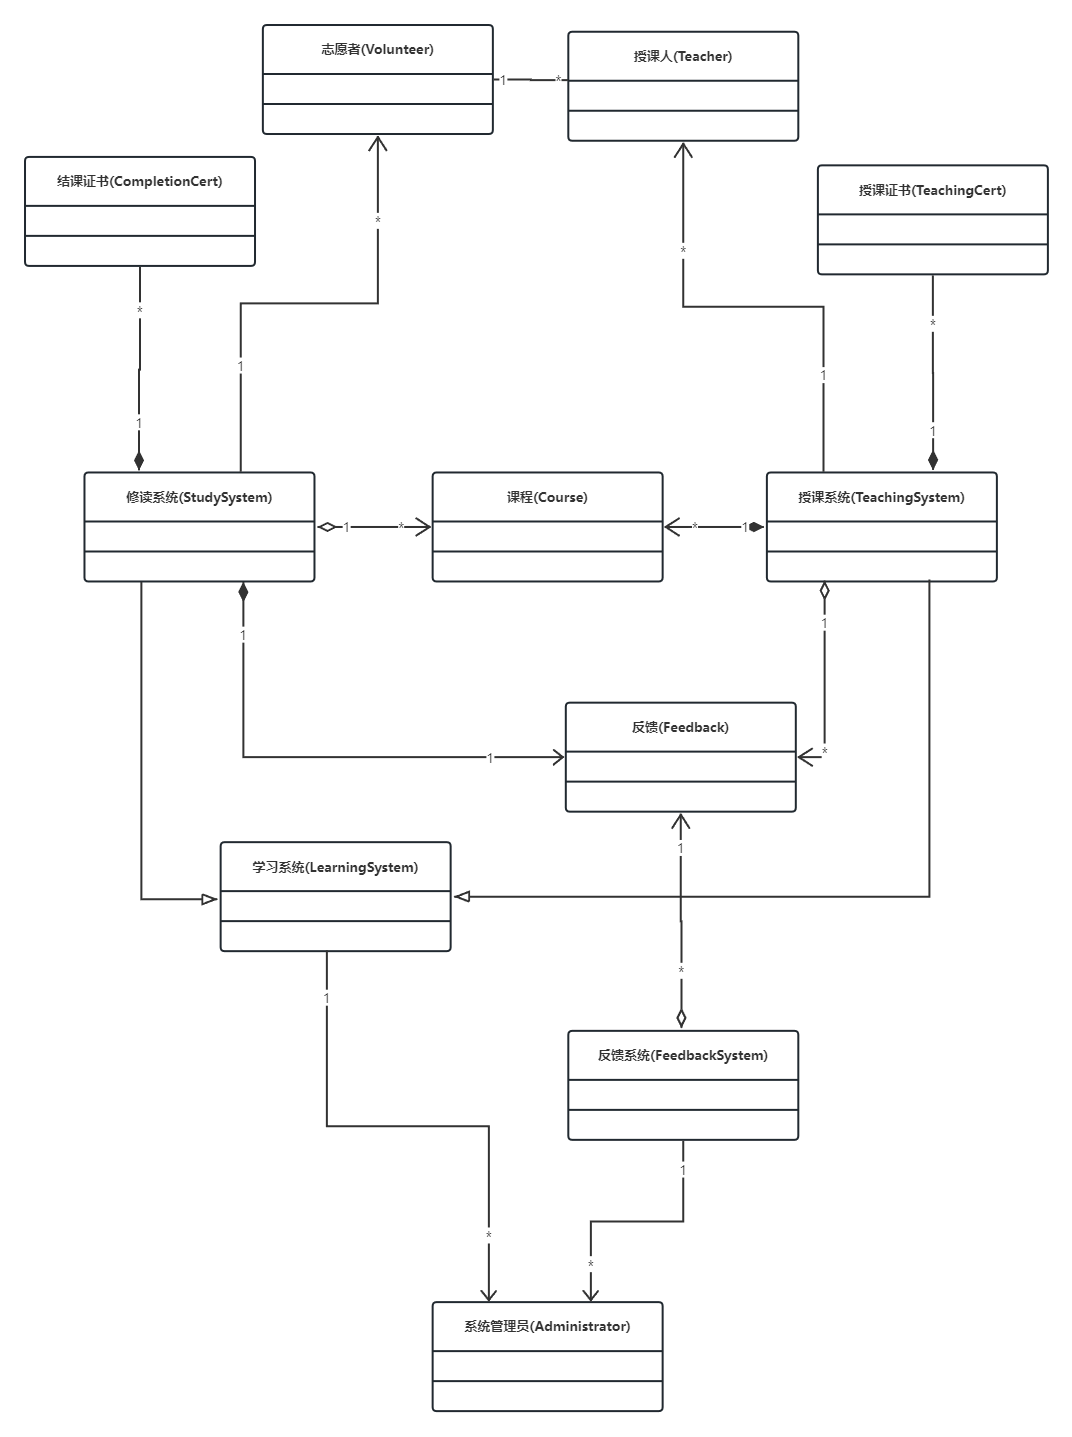
\includegraphics[scale=0.35]{OOA/fig/4-课程管理/课程管理类图.png}} 
    \bicaption{Volunet公益课程系统类图}{Class Diagram for Course System of Volunet} 
\end{figure}

\subsubsection{交流论坛系统类图}
\begin{figure}[H] 
    \center{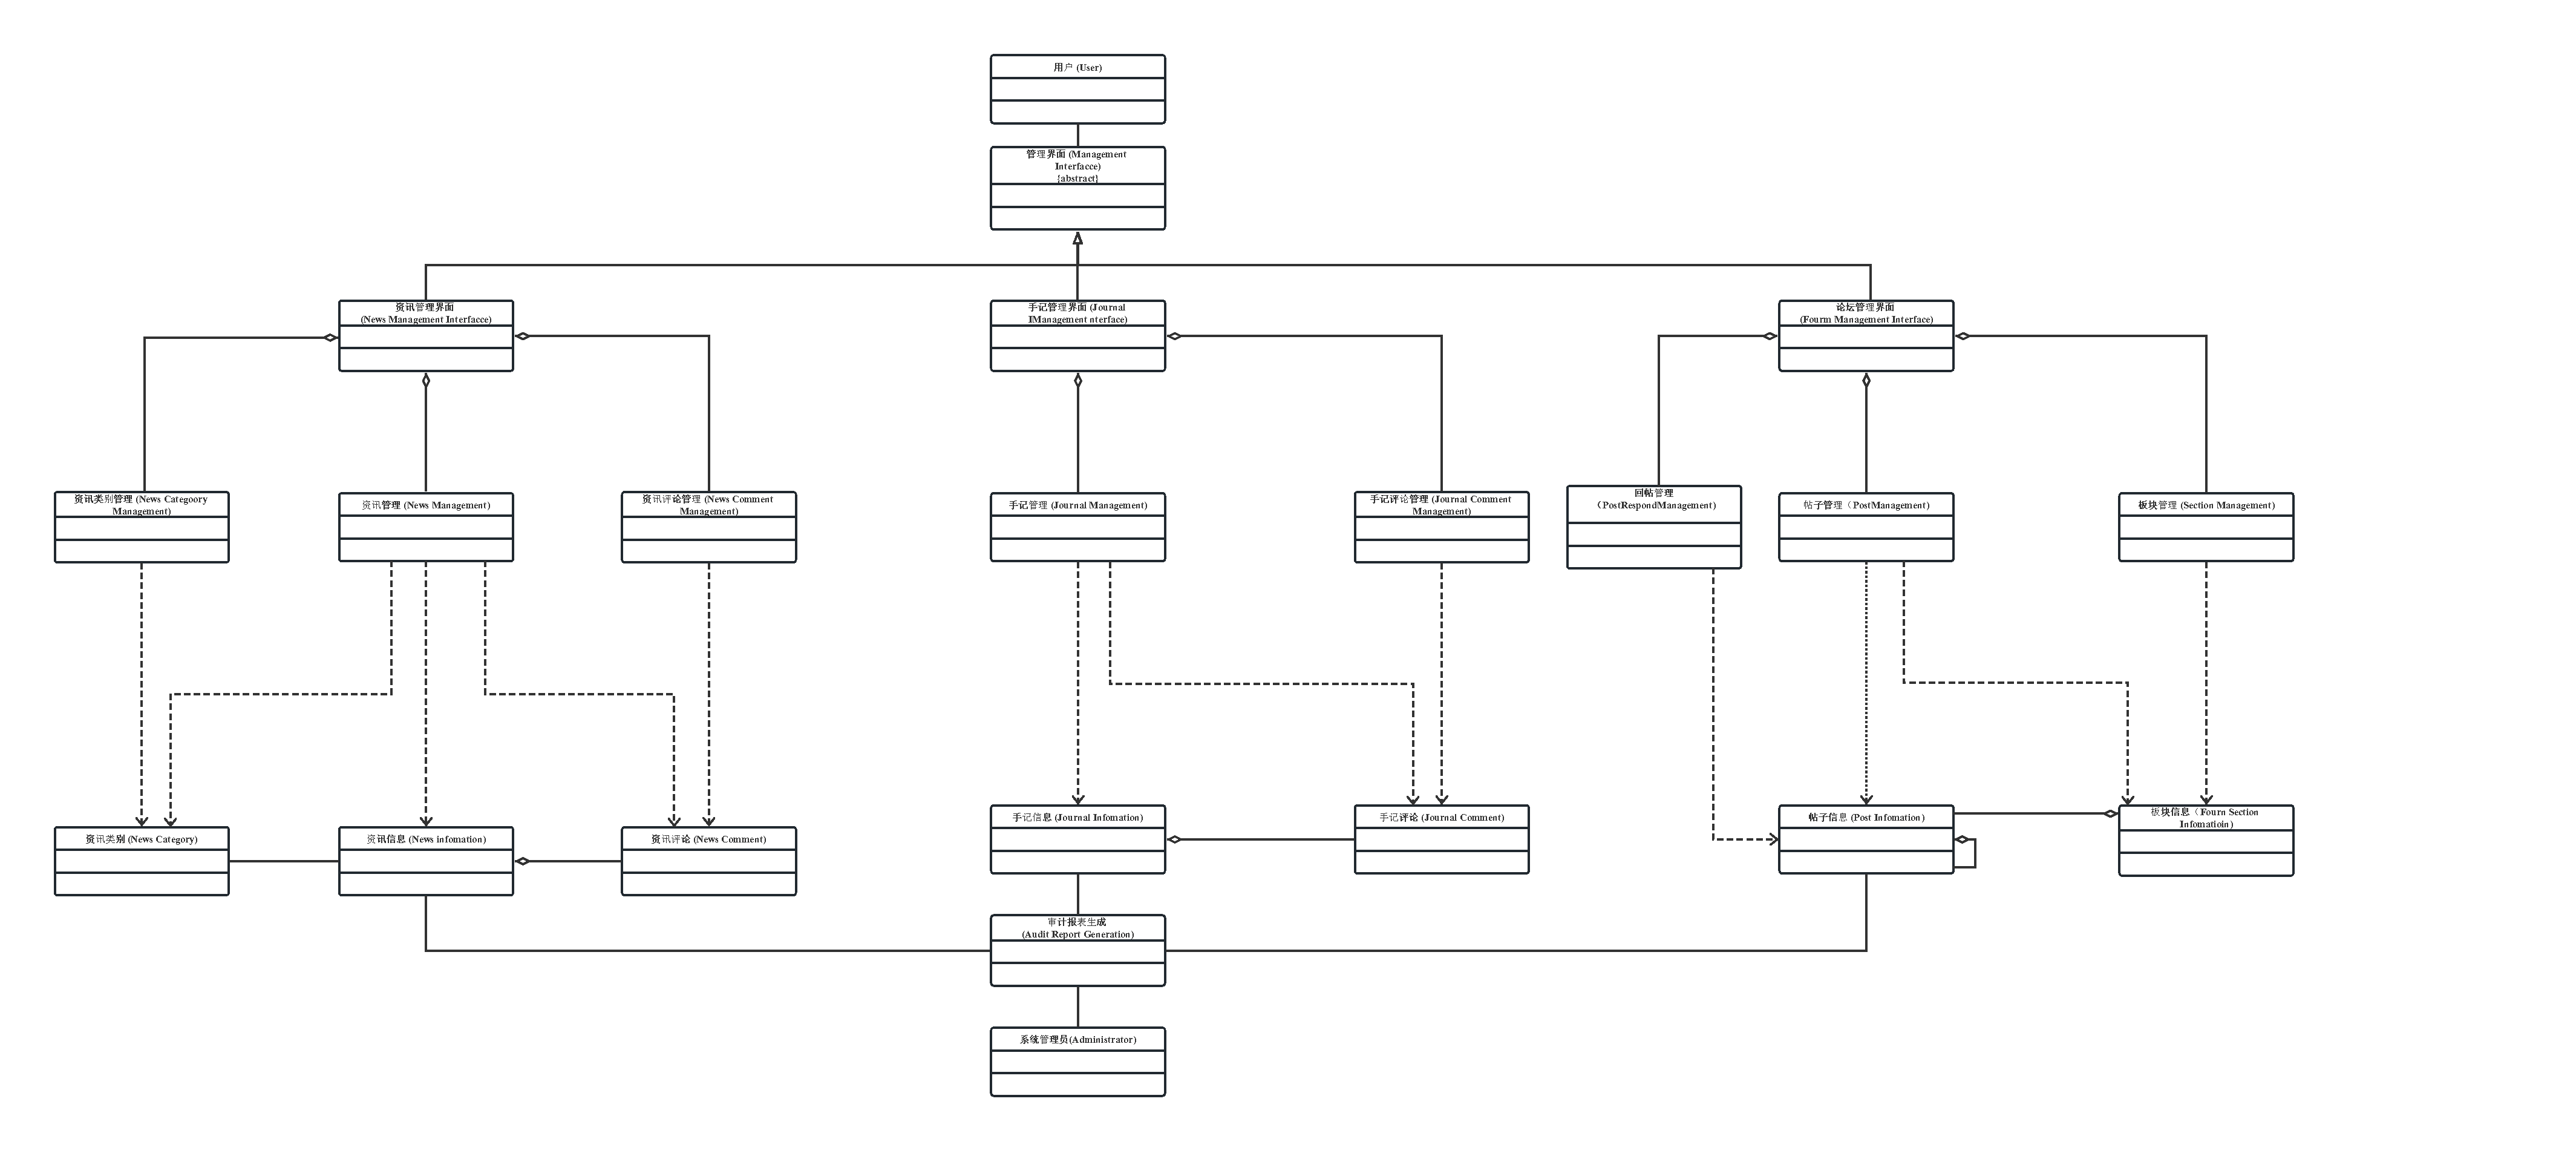
\includegraphics[scale=0.25, angle=90]{OOA/fig/5-论坛管理/论坛管理类图.pdf}} 
    \bicaption{Volunet交流论坛系统类图}{Class Diagram for Communication System of Volunet} 
\end{figure}

\subsubsection{志愿交友系统类图}
\begin{figure}[H] 
    \center{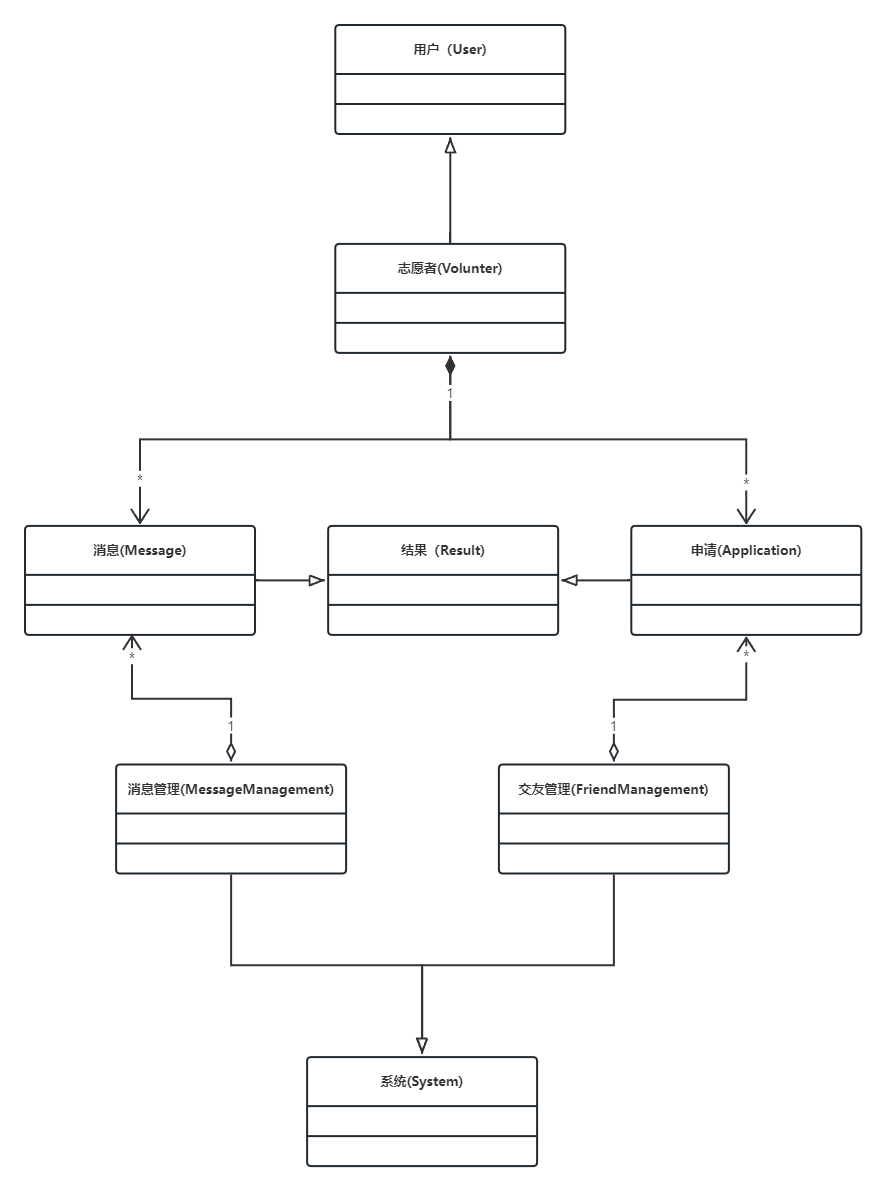
\includegraphics[scale=0.4]{OOA/fig/6-交友管理/志愿交友管理类图.png}} 
    \bicaption{Volunet志愿交友系统类图}{Class Diagram for Volunteer Friends System of Volunet} 
\end{figure}


\subsection{类的属性和操作}

\subsubsection{信息管理系统}

\paragraph{信息管理系统类属性与操作图}~{}
\begin{figure}[H] 
    \center{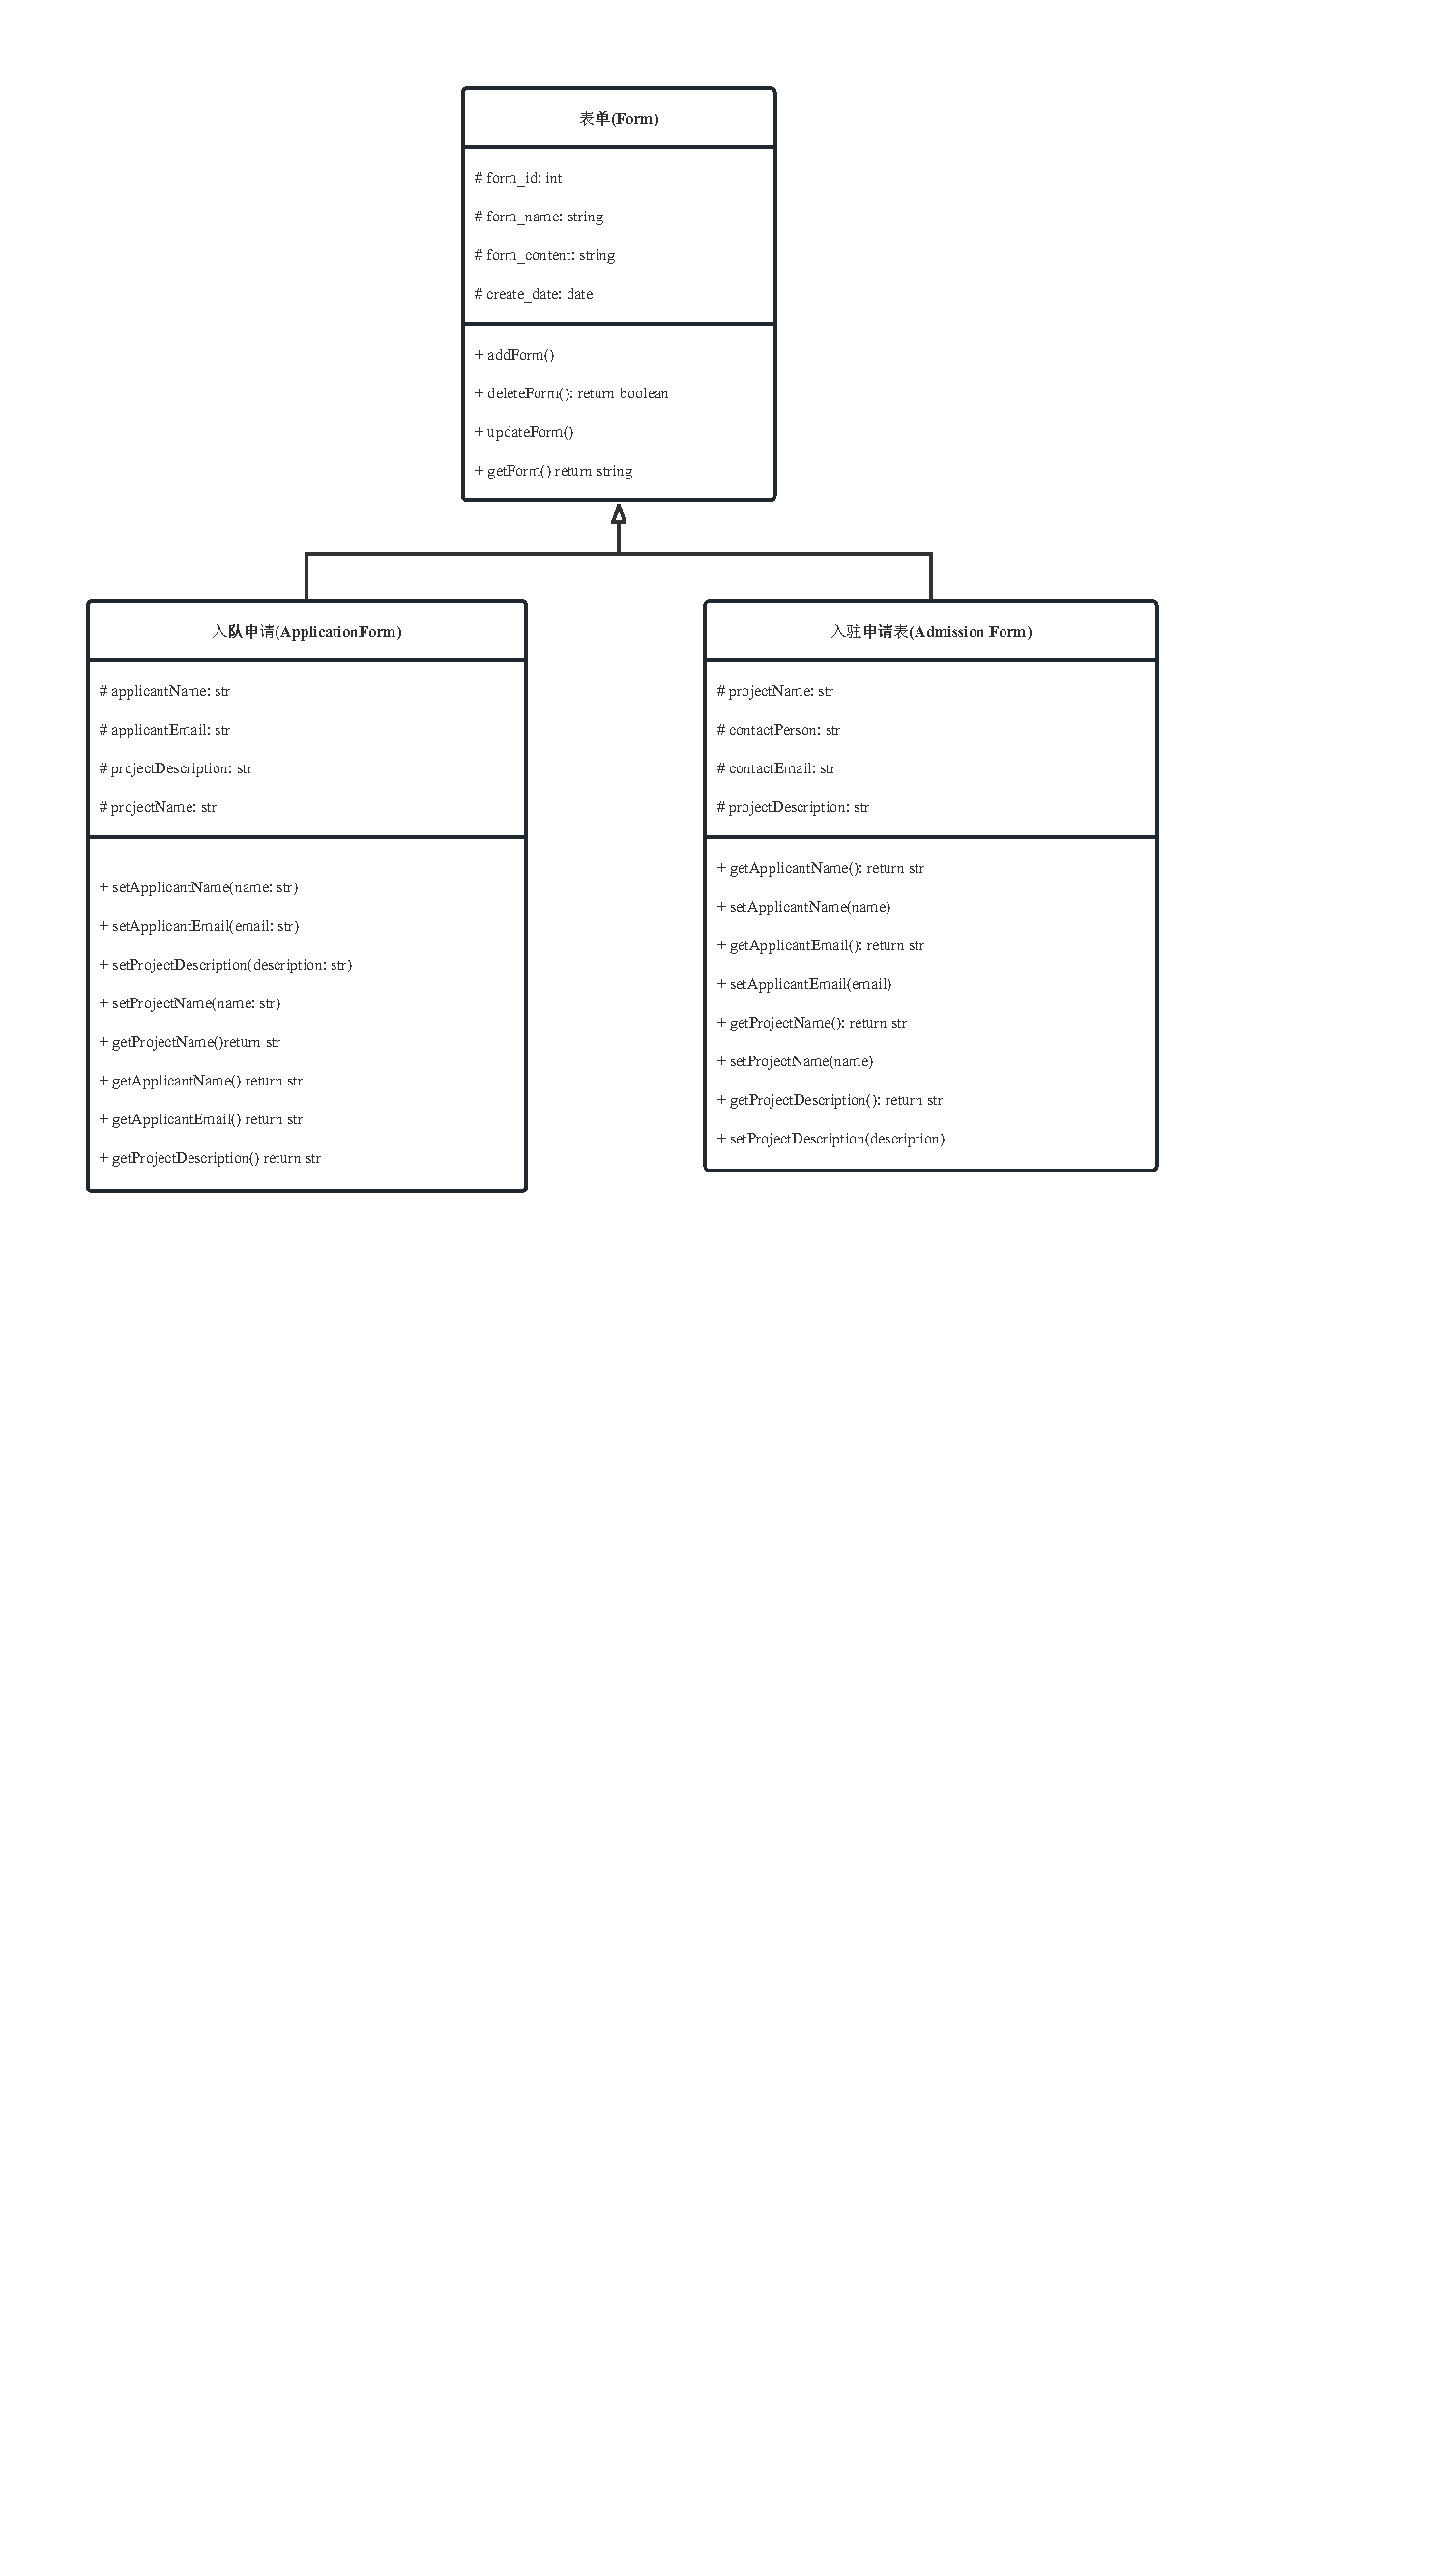
\includegraphics[scale=0.7]{OOA/fig/1-信息管理/信息管理类图-1.pdf}} 
    \bicaption{Volunet信息管理系统类属性与操作1子图}{Class Attributes and Operations Sub-Diagram 1 for Information Management System of Volunet} 
\end{figure}

\begin{figure}[H] 
    \center{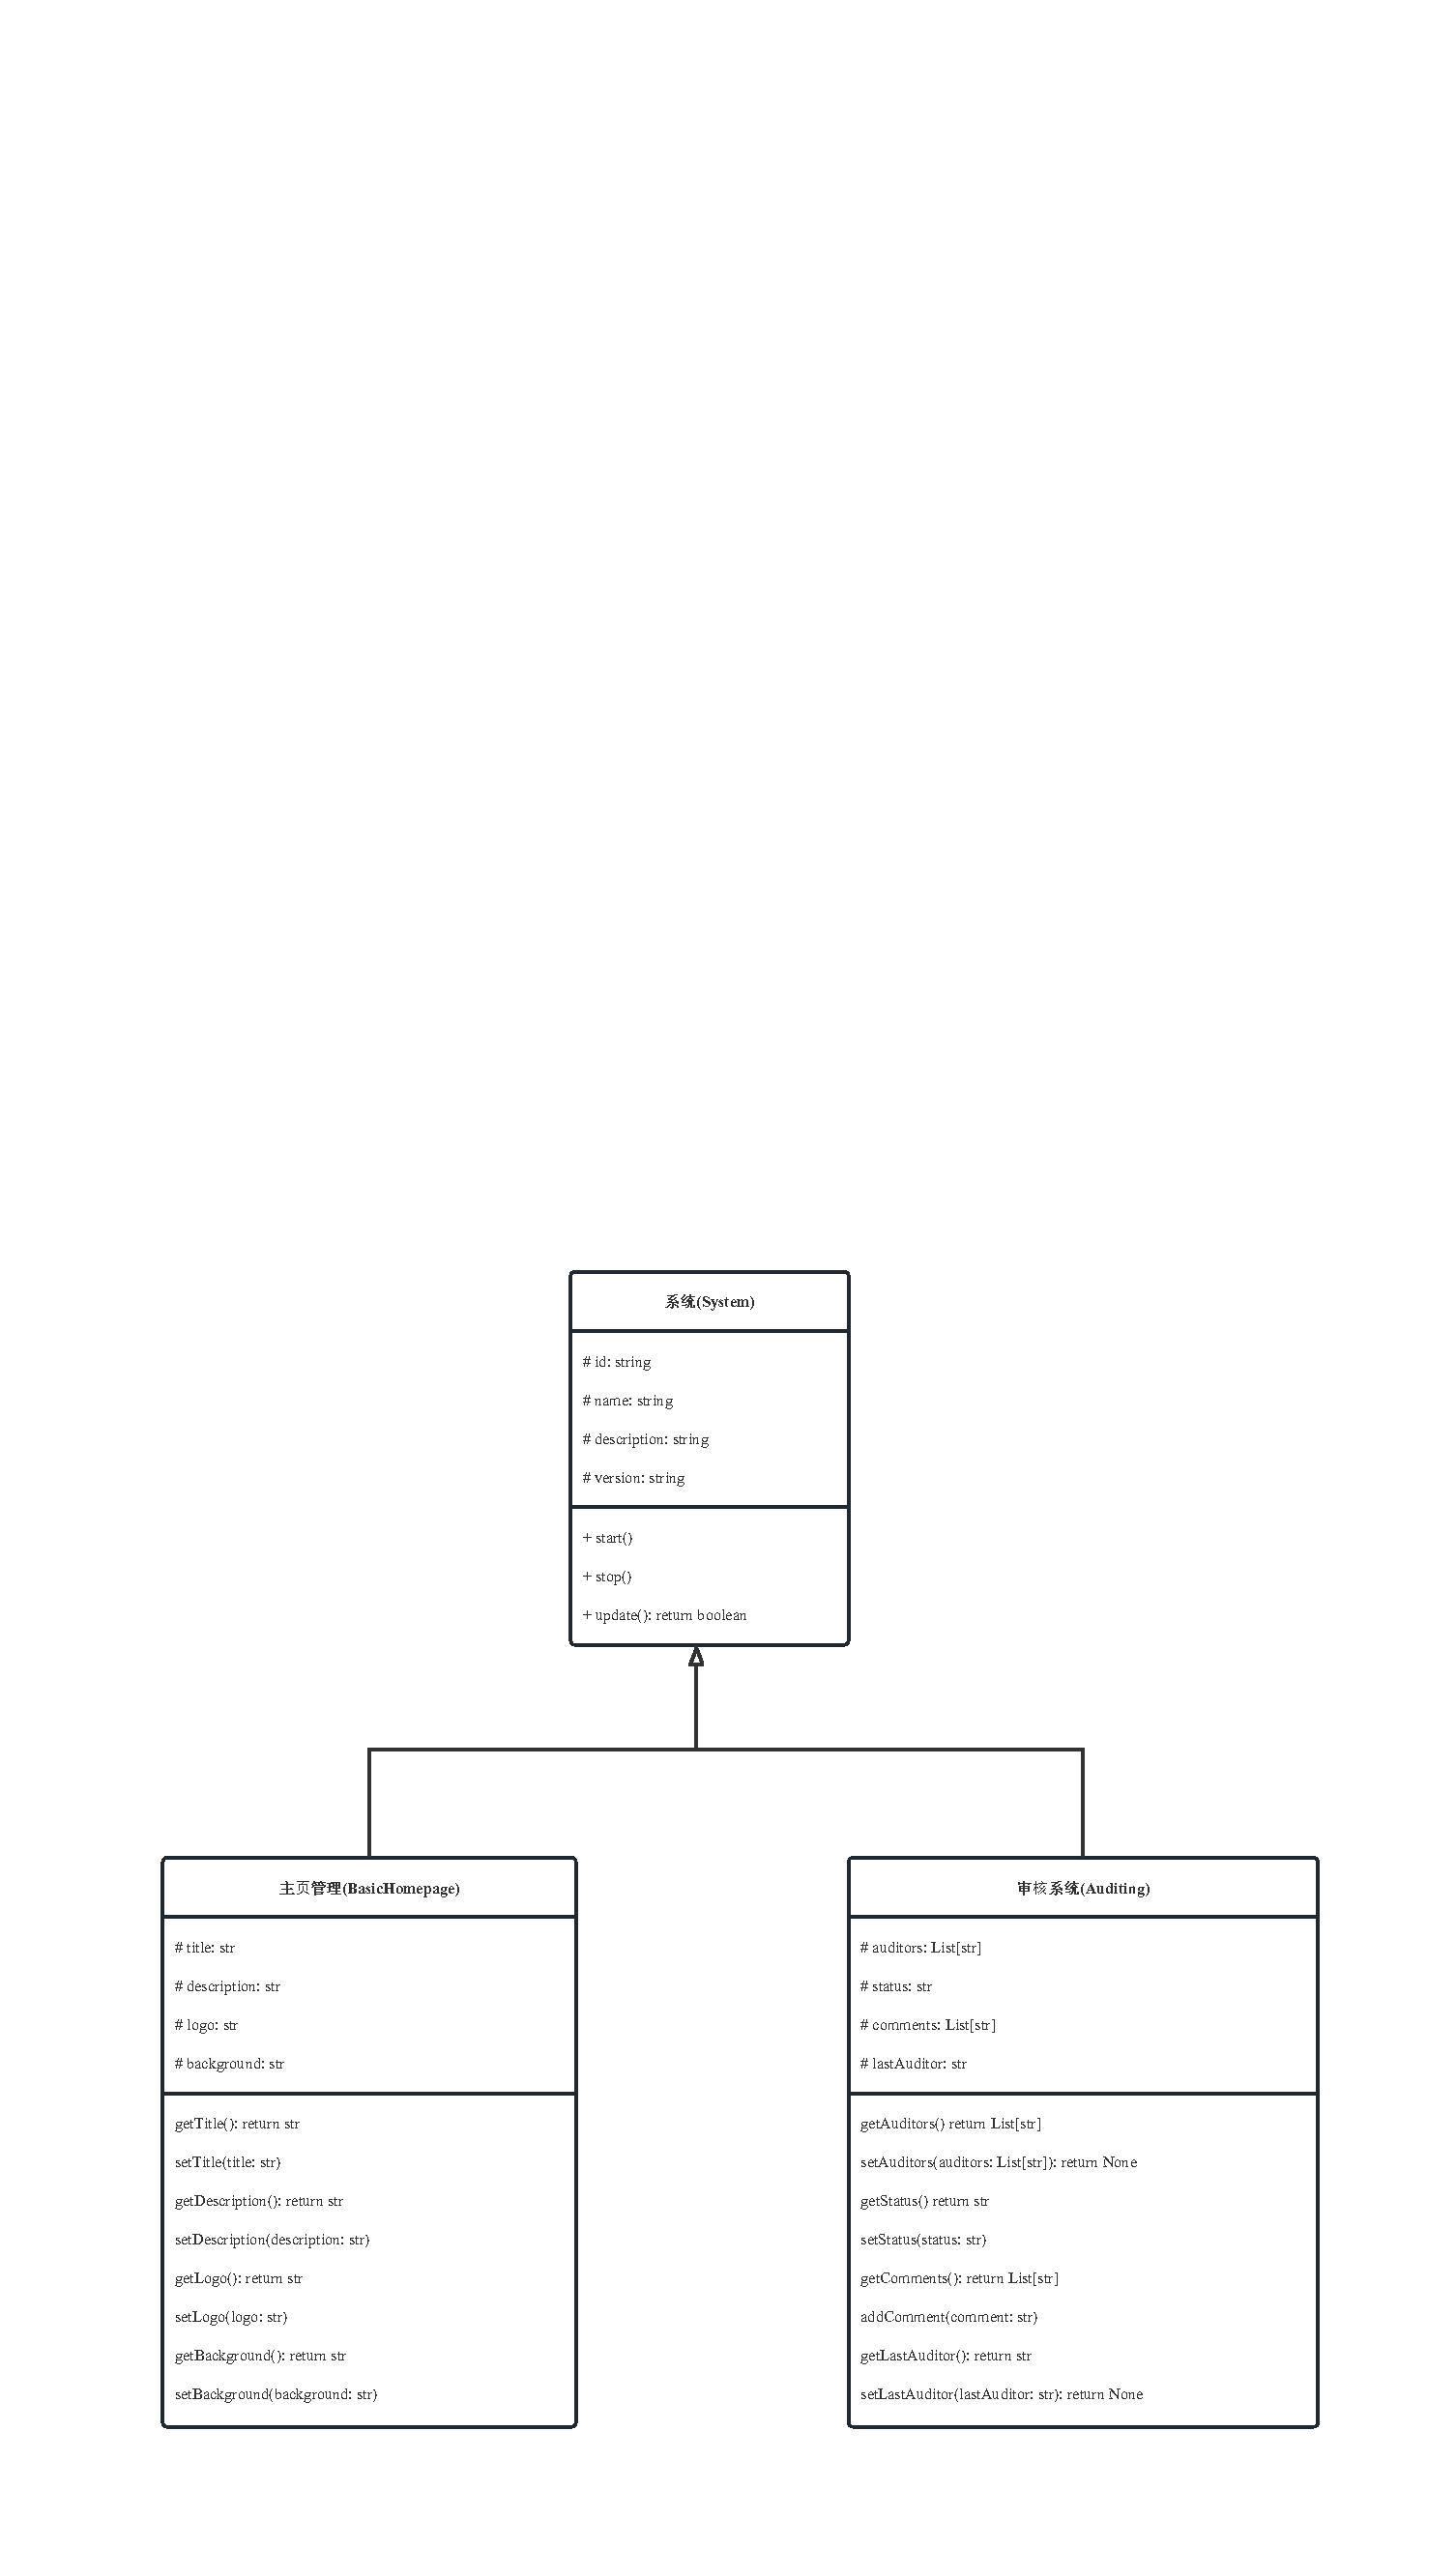
\includegraphics[scale=0.7]{OOA/fig/1-信息管理/信息管理类图-2.pdf}} 
    \bicaption{Volunet爱心捐助系统类属性与操作2子图}{Class Attributes and Operations Sub-Diagram 2 for Information Management System of Volunet} 
\end{figure}

\paragraph{信息管理系统类属性与操作描述}~{}

信息管理系统中类包含表单、入队申请、入驻申请表、系统、主页管理、审核系统,它们的属性与操作描述如下:

% 表单、入队申请、入驻申请表、系统、主页管理、审核系统
\begin{table}[H]  
\caption{“表单”类词条描述}  
\begin{center}  
    \begin{tabular}{l p{11cm}} 
        \hline
        \quad 名称:  &  表单 \\
        \hline
        \quad 编号:  & 1.1 \\
        \hline
        \quad 英文:  &  Form \\
        \hline
        \quad 简述:  & 用于收集、记录和处理信息的文档或工具 \\
        \hline
        \quad 属性:  & form\_id、form\_name、form\_content、create\_date: date\\
        \hline
        \quad 操作:  & addForm()、deleteForm()、updateForm()、getForm()\\
        \hline
        \quad 相关类:  & 入队申请、入驻申请表 \\
        \hline
    \end{tabular}
\end{center}
\end{table}

\begin{table}[H]  
\caption{“入队申请”类词条描述}  
\begin{center}  
    \begin{tabular}{l p{11cm}} 
        \hline
        \quad 名称:  &  入队申请 \\
        \hline
        \quad 编号:  & 1.2 \\
        \hline
        \quad 英文:  & ApplicationForm\\
        \hline
        \quad 简述:  & 用于申请加入某个志愿团队的表单 \\
        \hline
        \quad 属性:  & # applicantName、applicantEmail、projectDescription、projectName\\
        \hline
        \quad 操作:  & setApplicantName()、setApplicantEmail()、setProjectDescription()、 setProjectName()、getProjectName()、getApplicantName()、getApplicantEmail()、getProjectDescription()\\
        \hline
        \quad 相关类:  & 表单、志愿者。审核系统 \\
        \hline
    \end{tabular}
\end{center}
\end{table}

\begin{table}[H]  
\caption{“入驻申请表”类词条描述}  
\begin{center}  
    \begin{tabular}{l p{11cm}} 
        \hline
        \quad 名称:  &  入驻申请表 \\
        \hline
        \quad 编号:  & 1.3 \\
        \hline
        \quad 英文:  &  AdmissionForm \\
        \hline
        \quad 简述:  & 用于志愿团队申请入驻的表单 \\
        \hline
        \quad 属性:  & projectName、contactPerson、contactEmail、projectDescription\\
        \hline
        \quad 操作:  & + getApplicantName()、setApplicantName()、getApplicantEmail()、setApplicantEmail()、getProjectName()、setProjectName()、getProjectDescription()、setProjectDescription
\\
        \hline
        \quad 相关类:  & 表单、志愿团队、审核系统 \\
        \hline
    \end{tabular}
\end{center}
\end{table}

\begin{table}[H]  
\caption{“系统”类词条描述}  
\begin{center}  
    \begin{tabular}{l p{11cm}} 
        \hline
        \quad 名称:  &  系统 \\
        \hline
        \quad 编号:  & 1.4 \\
        \hline
        \quad 英文:  &  System \\
        \hline
        \quad 简述:  & 信息管理系统的简称 \\
        \hline
        \quad 属性:  & id、name、description、version\\
        \hline
        \quad 操作:  & start()、stop()、update()\\
        \hline
        \quad 相关类:  & 主页管理、审核系统 \\
        \hline
    \end{tabular}
\end{center}
\end{table}

\begin{table}[H]  
\caption{“主页管理”类词条描述}  
\begin{center}  
    \begin{tabular}{l p{11cm}} 
        \hline
        \quad 名称:  &  主页管理 \\
        \hline
        \quad 编号:  & 1.5 \\
        \hline
        \quad 英文:  &  BasicHomepage \\
        \hline
        \quad 简述:  & 负责对志愿者主页进行管理的系统 \\
        \hline
        \quad 属性:  & title、description、logo、background\\
        \hline
        \quad 操作:  & getTitle()、setTitle()、getDescription()、setDescription()、getLogo()、setLogo()、getBackground()、setBackground()\\
        \hline
        \quad 相关类:  & 系统、志愿者 \\
        \hline
    \end{tabular}
\end{center}
\end{table}

\begin{table}[H]  
\caption{“审核系统”类词条描述}  
\begin{center}  
    \begin{tabular}{l p{11cm}} 
        \hline
        \quad 名称:  &  审核系统 \\
        \hline
        \quad 编号:  & 1.6 \\
        \hline
        \quad 英文:  &  Auditing \\
        \hline
        \quad 简述:  & 负责信息审核的系统 \\
        \hline
        \quad 属性:  & auditors、status、comments、lastAuditor\\
        \hline
        \quad 操作:  & getAuditors()、setAuditors()、getStatus()、setStatus()、getComments()、addComment()、getLastAuditor()、setLastAuditor()
\\
        \hline
        \quad 相关类:  & 系统、系统管理员 \\
        \hline
    \end{tabular}
\end{center}
\end{table}

\subsubsection{志愿服务系统}

\paragraph{志愿服务系统类属性与操作图}~{}
\begin{figure}[H] 
    \center{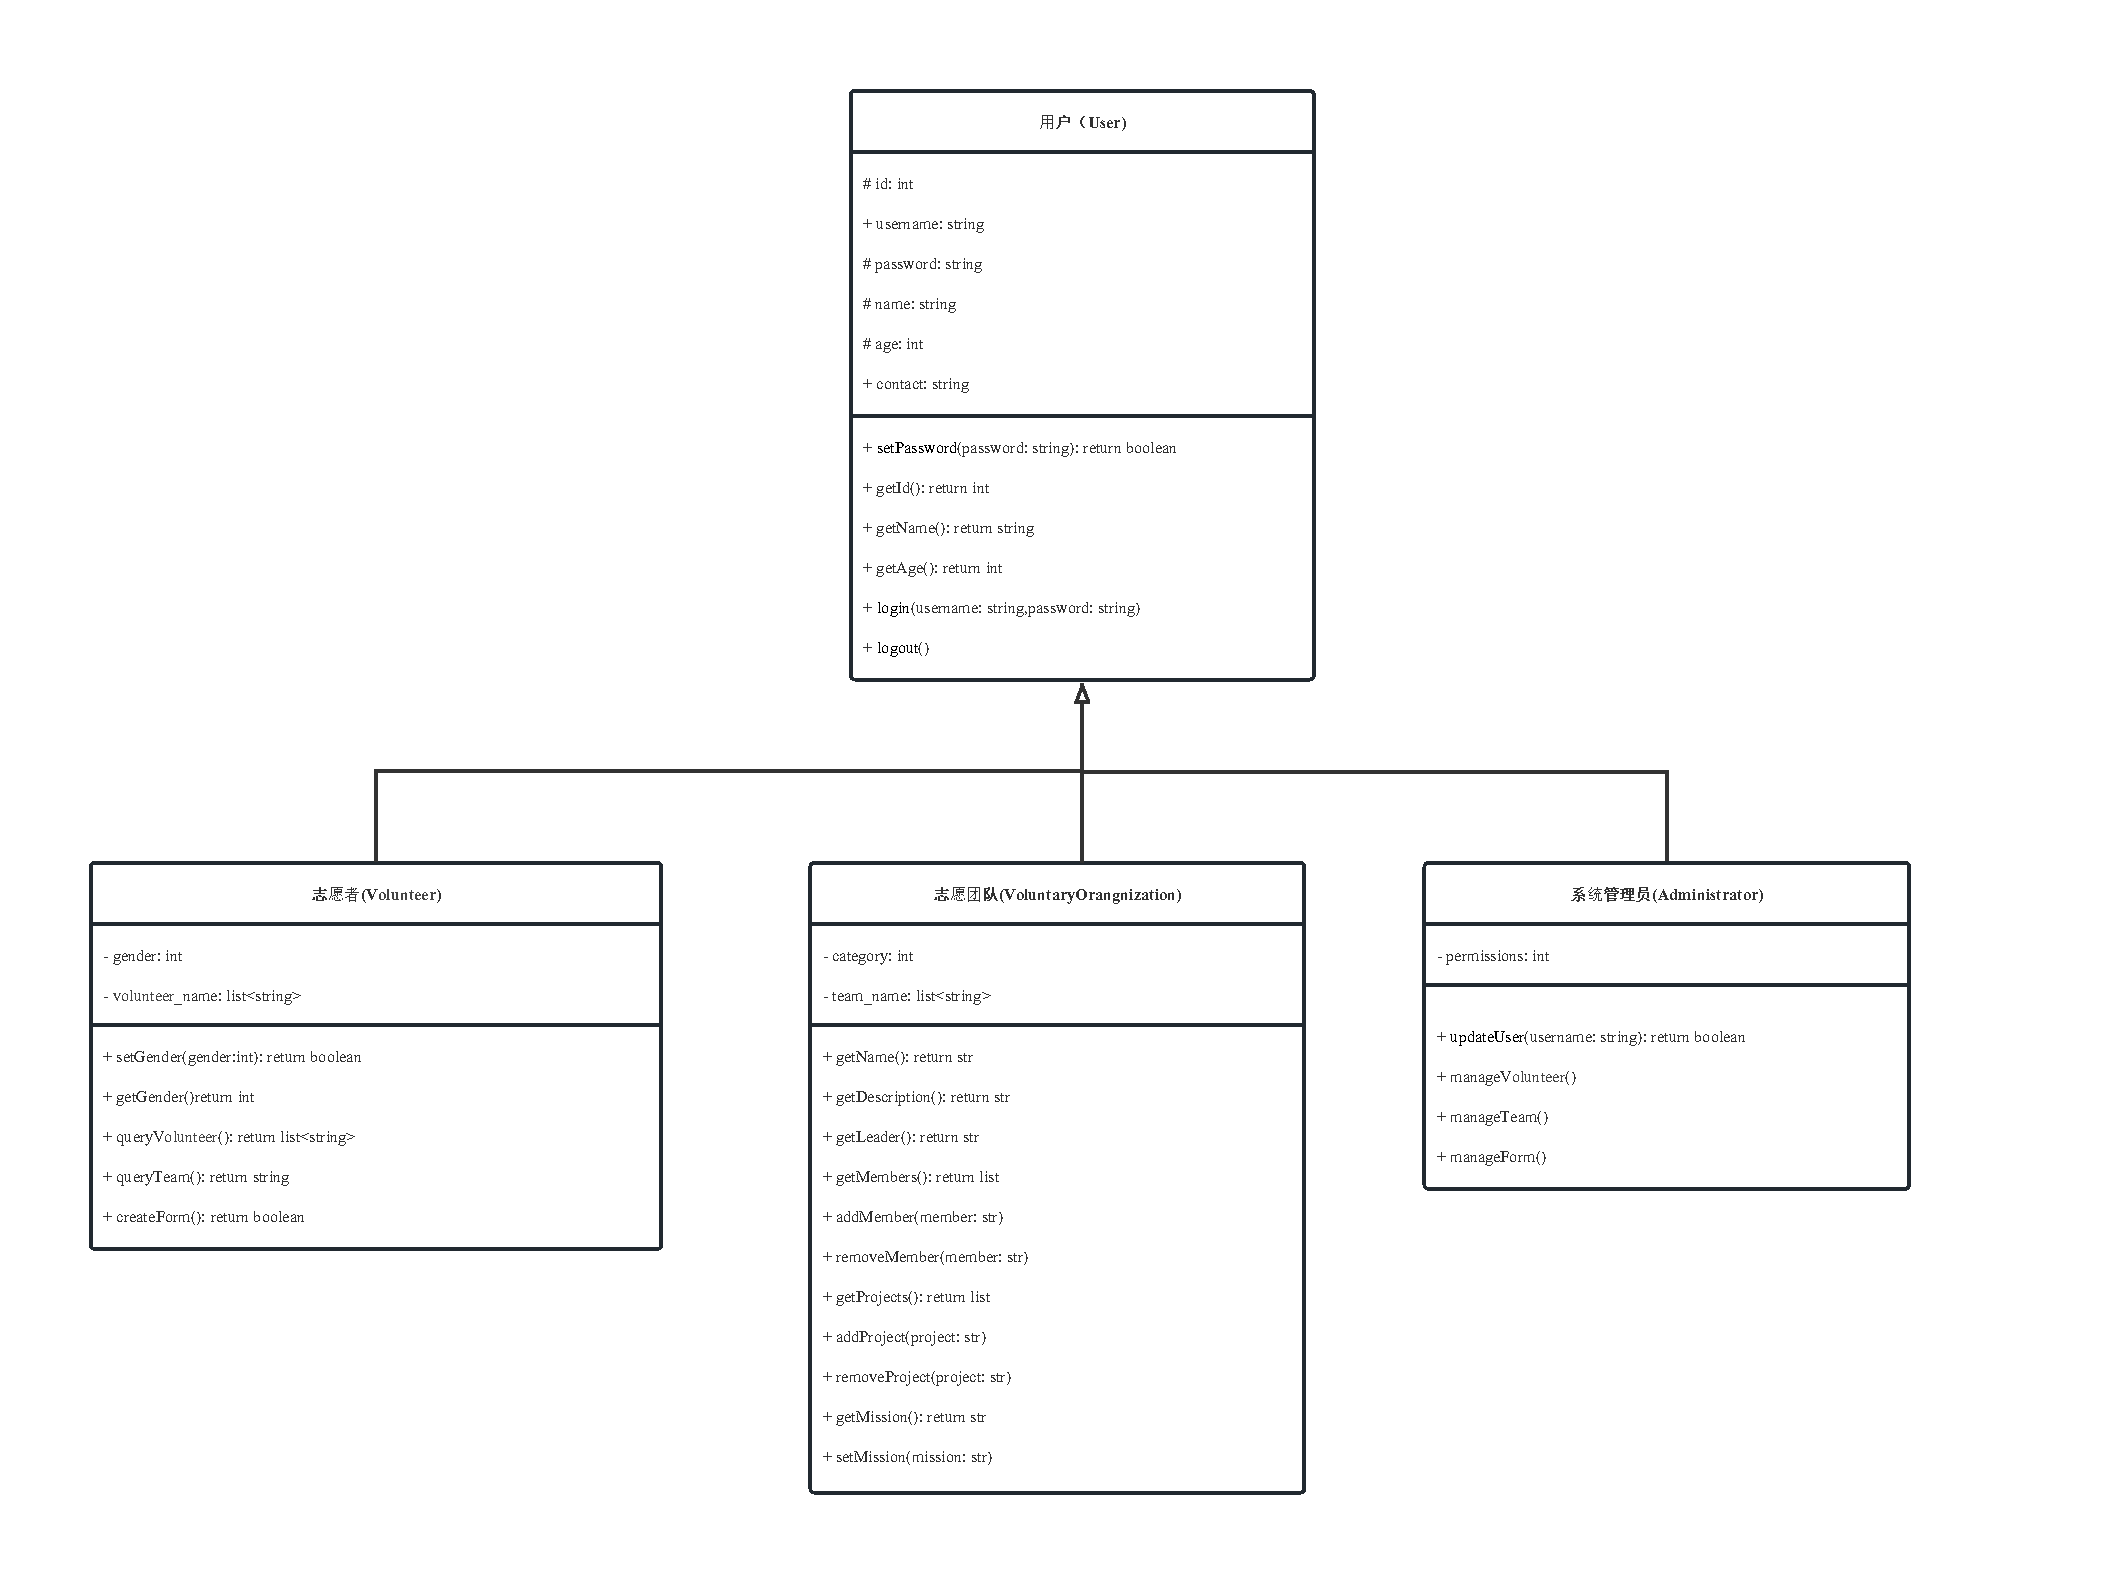
\includegraphics[scale=0.5]{OOA/fig/2-志愿服务/志愿服务类图-1.pdf}} 
    \bicaption{Volunet志愿服务系统类属性与操作1子图}{Class Attributes and Operations Sub-Diagram 1 for Volunteer Service System of Volunet} 
\end{figure}

\begin{figure}[H] 
    \center{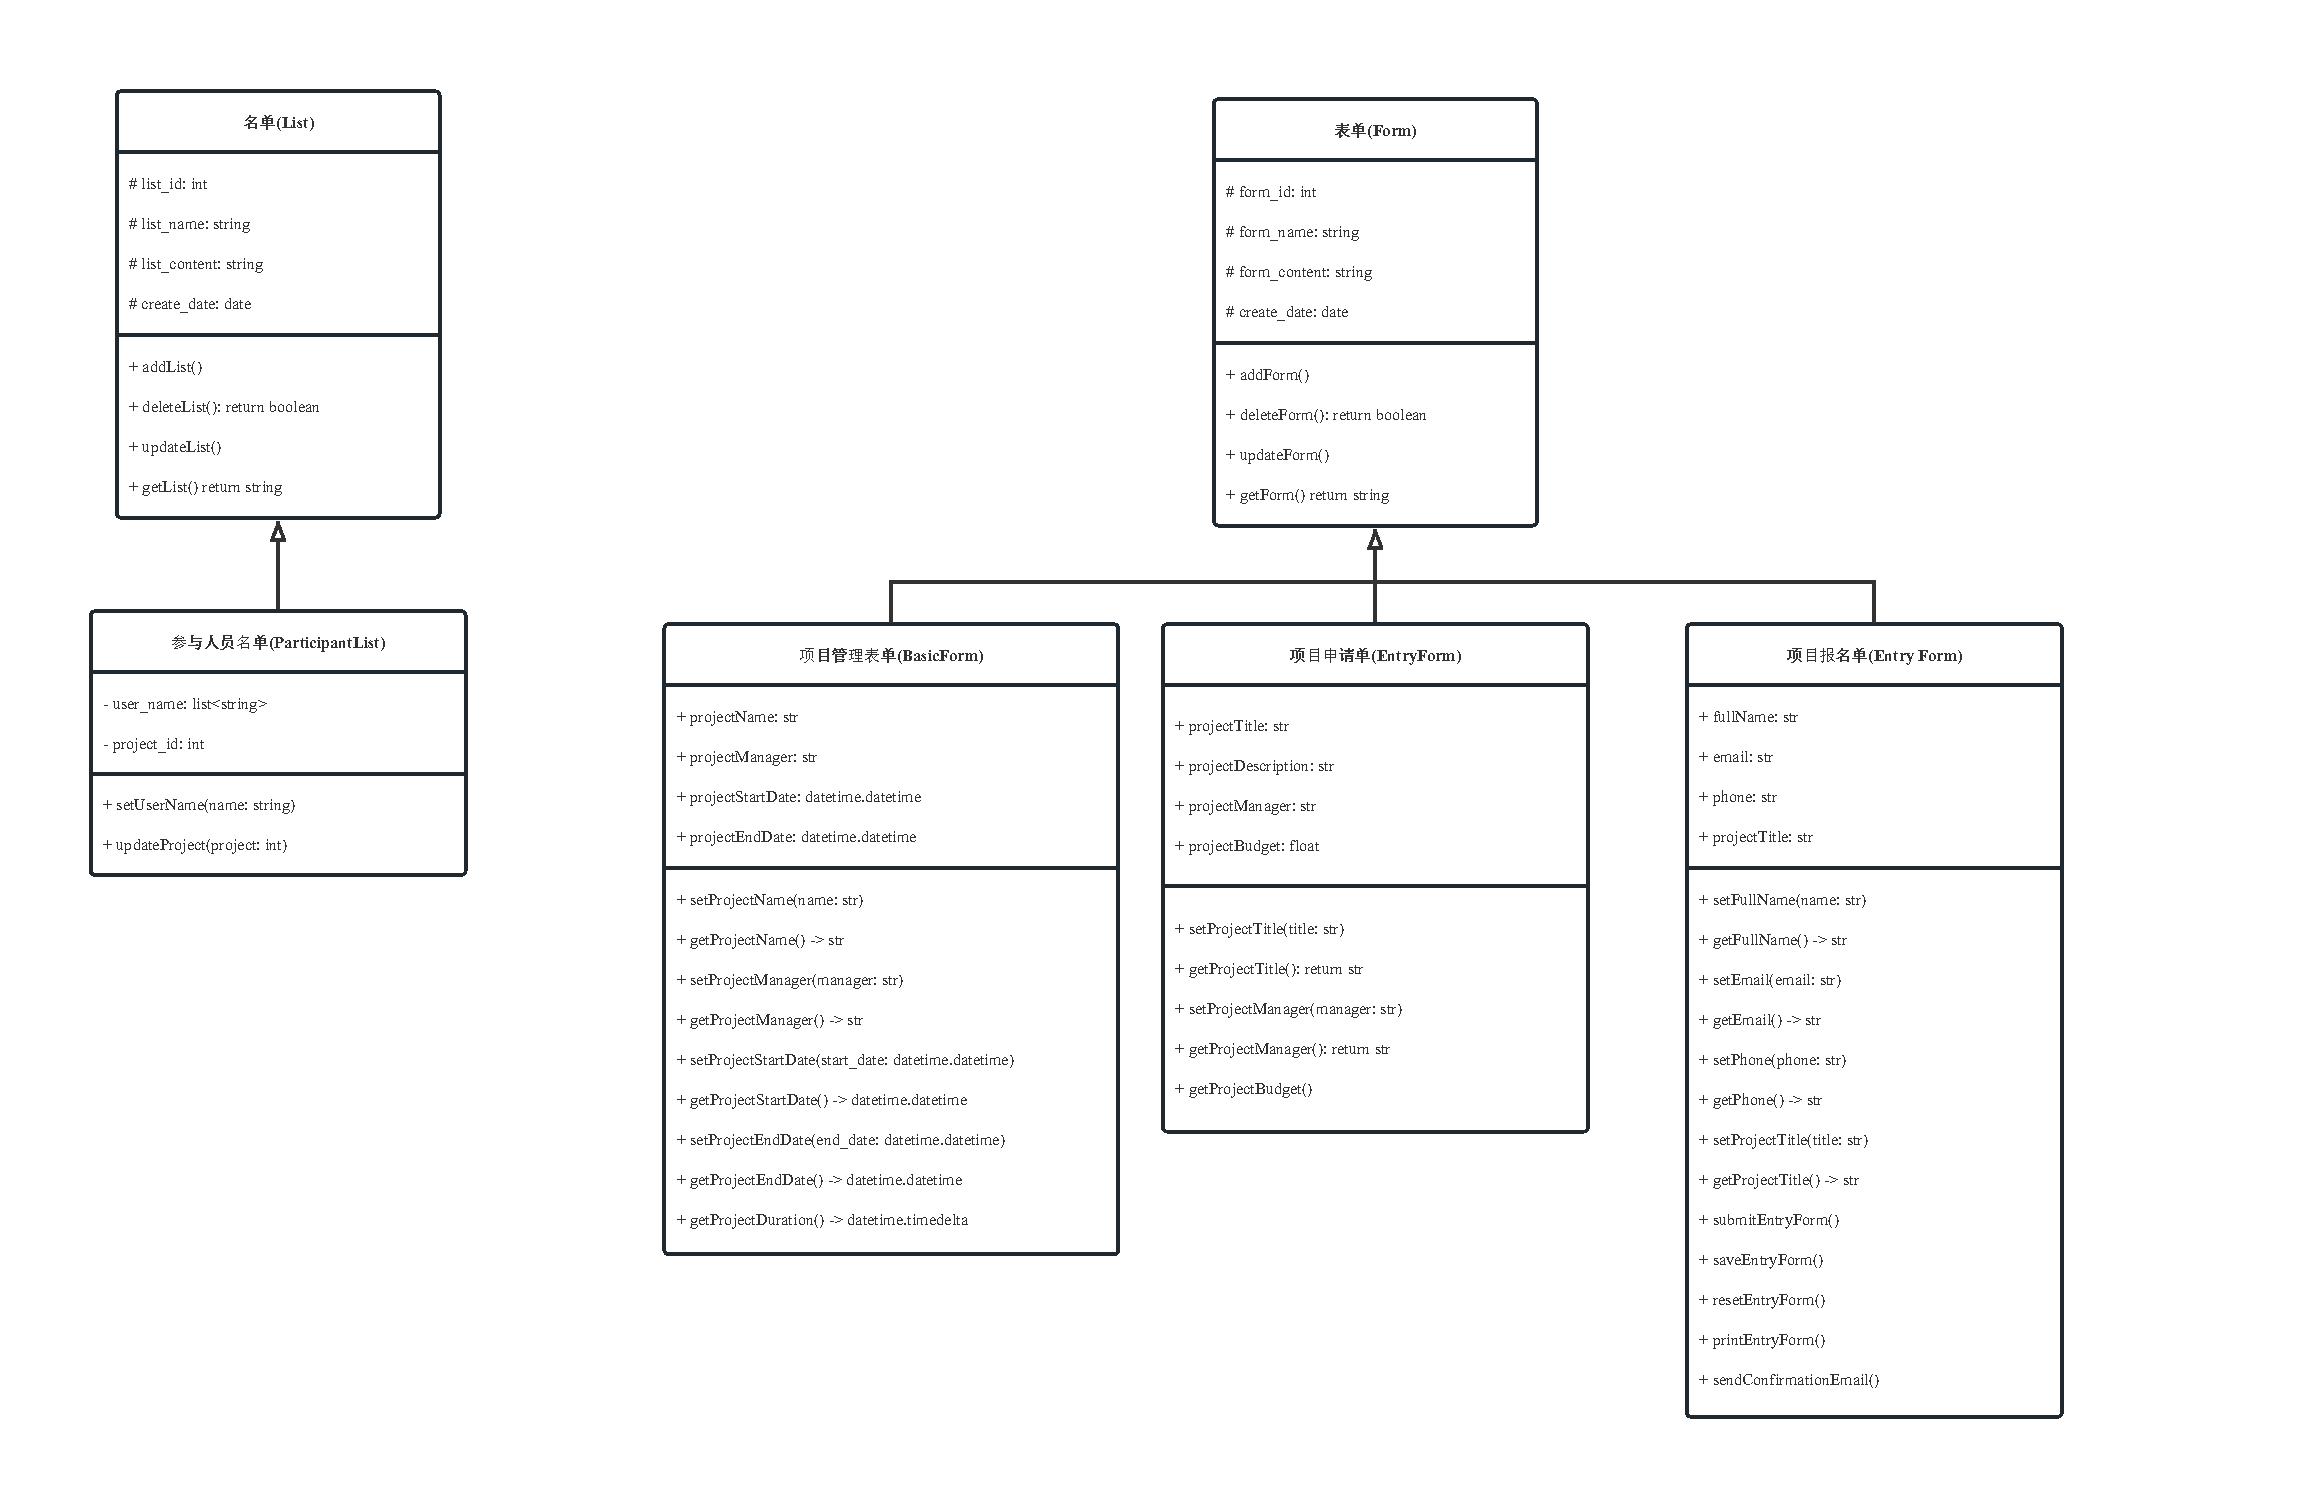
\includegraphics[scale=0.45]{OOA/fig/2-志愿服务/志愿服务类图-2.pdf}} 
    \bicaption{Volunet志愿服务系统类属性与操作2子图}{Class Attributes and Operations Sub-Diagram 2 for Volunteer Service System of Volunet} 
\end{figure}

\paragraph{志愿服务系统类属性与操作描述}~{}

志愿服务系统中类包含用户、志愿者、志愿团队、系统管理员、名单、参与人员名单、表单、项目申请单、项目报名单、项目管理表单,它们的属性与操作描述如下:

% 用户、志愿者、志愿团队、系统管理员、名单、参与人员名单、表单、
\begin{table}[H]  
\caption{“用户”类词条描述}  
\begin{center}  
    \begin{tabular}{l p{11cm}} 
        \hline
        \quad 名称:  &  用户 \\
        \hline
        \quad 编号:  & 2.1 \\
        \hline
        \quad 英文:  &  User \\
        \hline
        \quad 简述:  & 使用志愿服务系统的个人或组织的统称 \\
        \hline
        \quad 属性:  & id、username、password、name、age、contact \\
        \hline
        \quad 操作:  & setPassword()、getId()、getName()、getAge() 、login()、logout() \\
        \hline
        \quad 相关类:  & 志愿者、志愿团队、系统管理员 \\
        \hline
    \end{tabular}
\end{center}
\end{table}

\begin{table}[H]  
\caption{“志愿团队”类词条描述}  
\begin{center}  
    \begin{tabular}{l p{11cm}} 
        \hline
        \quad 名称:  &  志愿团队 \\
        \hline
        \quad 编号:  & 2.2 \\
        \hline
        \quad 英文:  &  Team \\
        \hline
        \quad 简述:  & 使用志愿服务系统发布志愿项目的组织 \\
        \hline
        \quad 属性:  & category、team\_name \\
        \hline 
        \quad 操作:  & getName()、getDescription()、getLeader()、getMembers()、addMember()、removeMember()、getProjects()、addProject()、removeProject()、getMission()、setMission()
\\
        \hline
        \quad 相关类:  & 用户、项目申请单、志愿者 \\
        \hline
    \end{tabular}
\end{center}
\end{table}

\begin{table}[H]  
\caption{“志愿者”类词条描述}  
\begin{center}  
    \begin{tabular}{l p{11cm}} 
        \hline
        \quad 名称:  &  志愿者 \\
        \hline
        \quad 编号:  & 2.3 \\
        \hline
        \quad 英文:  &  Volunteer \\
        \hline
        \quad 简述:  & 使用志愿服务系统对参与志愿项目的人 \\
        \hline
        \quad 属性:  & gender、volunteer\_name
 \\
        \hline
        \quad 操作:  & setGender()、getGender()、queryVolunteer()、queryTeam()、createForm()
 \\
        \hline
        \quad 相关类:  & 用户、志愿团队、项目报名单 \\
        \hline
    \end{tabular}
\end{center}
\end{table}

\begin{table}[H]  
\caption{“系统管理员”类词条描述}  
\begin{center}  
    \begin{tabular}{l p{11cm}} 
        \hline
        \quad 名称:  &  系统管理员 \\
        \hline
        \quad 编号:  & 2.4 \\
        \hline
        \quad 英文:  &  Administrator \\
        \hline
        \quad 简述:  & 管理志愿服务系统,进行信息审核的人 \\
        \hline
        \quad 属性:  & permissions \\
        \hline
        \quad 操作:  & updateUser()、manageVolunteer()、manageTeam()、manageForm()\\
        \hline
        \quad 相关类:  & 用户、审核系统\\
        \hline
    \end{tabular}
\end{center}
\end{table}

\begin{table}[H]  
\caption{“名单”类词条描述}  
\begin{center}  
    \begin{tabular}{l p{11cm}} 
        \hline
        \quad 名称:  &  名单 \\
        \hline
        \quad 编号:  & 2.5 \\
        \hline
        \quad 英文:  &  List \\
        \hline
        \quad 简述:  & 按照一定标准或规则列出的人员或事物清单 \\
        \hline
        \quad 属性:  &list\_id、list\_name、list\_content、create\_date\\
        \hline
        \quad 操作:  & addList()、deleteList()、updateList()、getList() \\
        \hline
        \quad 相关类:  & 参与人员名单 \\
        \hline
    \end{tabular}
\end{center}
\end{table}

\begin{table}[H]  
\caption{“参与人员名单”类词条描述}  
\begin{center}  
    \begin{tabular}{l p{11cm}} 
        \hline
        \quad 名称:  &  参与人员名单 \\
        \hline
        \quad 编号:  & 2.6 \\
        \hline
        \quad 英文:  &  ParticipantList \\
        \hline
        \quad 简述:  & 参与志愿项目的公示名单 \\
        \hline
        \quad 属性:  & user\_name、project\_id
\\
        \hline
        \quad 操作:  & setUserName()、updateProject()

\\
        \hline
        \quad 相关类:  & 名单、志愿团队 \\
        \hline
    \end{tabular}
\end{center}
\end{table}

\begin{table}[H]  
\caption{“表单”类词条描述}  
\begin{center}  
    \begin{tabular}{l p{11cm}} 
        \hline
        \quad 名称:  &  表单 \\
        \hline
        \quad 编号:  & 2.7 \\
        \hline
        \quad 英文:  &  Form \\
        \hline
        \quad 简述:  & 用于收集、记录和处理信息的文档或工具 \\
        \hline
        \quad 属性:  & form\_id、form\_name、form\_content、create\_date: date\\
        \hline
        \quad 操作:  & addForm()、deleteForm()、updateForm()、getForm()\\
        \hline
        \quad 相关类:  & 项目申请单、项目报名单、项目管理名单 \\
        \hline
    \end{tabular}
\end{center}
\end{table}

\begin{table}[H]  
\caption{“项目申请单”类词条描述}  
\begin{center}  
    \begin{tabular}{l p{11cm}} 
        \hline
        \quad 名称:  &  项目申请单 \\
        \hline
        \quad 编号:  & 2.8 \\
        \hline
        \quad 英文:  & EntryForm\\
        \hline
        \quad 简述:  & 用于提交和审批志愿项目计划的表单 \\
        \hline
        \quad 属性:  & projectTitle、projectDescription、projectManager、projectBudget\\
        \hline
        \quad 操作:  & setProjectTitle()、getProjectTitle()、setProjectManager()、getProjectManager()、getProjectBudget()\\
        \hline
        \quad 相关类:  & 表单、系统管理员、志愿团队 \\
        \hline
    \end{tabular}
\end{center}
\end{table}

\begin{table}[H]  
\caption{“项目报名单”类词条描述}  
\begin{center}  
    \begin{tabular}{l p{11cm}} 
        \hline
        \quad 名称:  &  项目报名单 \\
        \hline
        \quad 编号:  & 2.9 \\
        \hline
        \quad 英文:  &  EntryForm \\
        \hline
        \quad 简述:  & 收集志愿项目参与者信息的表单 \\
        \hline
        \quad 属性:  & fullName、email、phone、projectTitle\\
        \hline
        \quad 操作:  & setFullName()、getFullName()、setEmail()、getEmail()、setPhone()、getPhone()、setProjectTitle(title: str)、getProjectTitle()、submitEntryForm()、saveEntryForm()、resetEntryForm()、printEntryForm()、sendConfirmationEmail()
\\
        \hline
        \quad 相关类:  & 表单、志愿者、系统管理员 \\
        \hline
    \end{tabular}
\end{center}
\end{table}

\begin{table}[H]  
\caption{“项目管理表单”类词条描述}  
\begin{center}  
    \begin{tabular}{l p{11cm}} 
        \hline
        \quad 名称:  &  项目管理表单 \\
        \hline
        \quad 编号:  & 2.10 \\
        \hline
        \quad 英文:  &  BasicForm \\
        \hline
        \quad 简述:  & 用于记录和跟踪志愿项目管理信息的表单 \\
        \hline
        \quad 属性:  & projectName、projectManager、projectStartDate、projectEndDate\\
        \hline
        \quad 操作:  & setProjectName()、getProjectName()、setProjectManager()、getProjectManager()、setProjectStartDate()、getProjectStartDate()、setProjectEndDate()、getProjectEndDate()、getProjectDuration()\\
        \hline
        \quad 相关类:  & 志愿者、志愿团队、表单 \\
        \hline
    \end{tabular}
\end{center}
\end{table}


\subsubsection{爱心捐助系统}

\paragraph{爱心捐助系统类属性与操作图}~{}
\begin{figure}[H] 
    \center{\includegraphics[scale=0.3, angle=-90]{OOA/fig/3-爱心管理/爱心管理类图-2.pdf}} 
    \bicaption{Volunet爱心捐助系统类属性与操作1子图}{Class Attributes and Operations Sub-Diagram 1 for Love Donation System of Volunet} 
\end{figure}

\begin{figure}[H] 
    \center{\includegraphics[scale=0.35]{OOA/fig/3-爱心管理/爱心管理类图-3.pdf}} 
    \bicaption{Volunet爱心捐助系统类属性与操作2子图}{Class Attributes and Operations Sub-Diagram 2 for Love Donation System of Volunet} 
\end{figure}

\paragraph{爱心捐助系统类属性与操作描述}~{}

爱心捐助系统中类包含用户、捐款者、志愿团队、购买者、公益商户、系统管理员、订单、证书、爱心证书、名单、鸣谢名单、系统、授课系统、订单系统、捐款系统以及爱心反馈系统,它们的属性与操作描述如下:

% 捐款者、志愿团队、购买者、公益商户、系统管理员、订单、证书、爱心证书、名单、鸣谢名单、系统、授课系统、订单系统、捐款系统以及爱心反馈系统
\begin{table}[H]  
\caption{“用户”类词条描述}  
\begin{center}  
    \begin{tabular}{l p{11cm}} 
        \hline
        \quad 名称:  &  用户 \\
        \hline
        \quad 编号:  & 3.1 \\
        \hline
        \quad 英文:  &  User \\
        \hline
        \quad 简述:  & 使用爱心捐助系统的个人或组织的统称 \\
        \hline
        \quad 属性:  & id、username、password、name、age、contact \\
        \hline
        \quad 操作:  & setPassword()、getId()、getName()、getAge() 、login()、logout() \\
        \hline
        \quad 相关类:  & 捐款者、志愿团队、购买者、公益商户、系统管理员 \\
        \hline
    \end{tabular}
\end{center}
\end{table}

\begin{table}[H]  
\caption{“志愿团队”类词条描述}  
\begin{center}  
    \begin{tabular}{l p{11cm}} 
        \hline
        \quad 名称:  &  志愿团队 \\
        \hline
        \quad 编号:  & 3.2 \\
        \hline
        \quad 英文:  &  Team \\
        \hline
        \quad 简述:  & 使用爱心捐助系统接收项目捐助的组织 \\
        \hline
        \quad 属性:  & category、team\_name \\
        \hline 
        \quad 操作:  & setProject()、getProject()、queryProject()、queryDonor()、queryDonation()、applyCourse()、getProjectAnalysis()、modifyProject()、getLoveFeedback()\\
        \hline
        \quad 相关类:  & 用户、捐款系统 \\
        \hline
    \end{tabular}
\end{center}
\end{table}

\begin{table}[H]  
\caption{“捐款者”类词条描述}  
\begin{center}  
    \begin{tabular}{l p{11cm}} 
        \hline
        \quad 名称:  &  捐款者 \\
        \hline
        \quad 编号:  & 3.3 \\
        \hline
        \quad 英文:  &  Donor \\
        \hline
        \quad 简述:  & 使用爱心捐助系统对项目进行捐款的人 \\
        \hline
        \quad 属性:  & category、donor\_name\\
        \hline
        \quad 操作:  & setGender()、getGender()、queryTeam()、queryProject()、submitDonation()、queryDonation()、queryCertificate()、queryAcknowledgementList()、\\
        \hline
        \quad 相关类:  & 用户、捐款系统、爱心证书 \\
        \hline
    \end{tabular}
\end{center}
\end{table}

\begin{table}[H]  
\caption{“购买者”类词条描述}  
\begin{center}  
    \begin{tabular}{l p{11cm}} 
        \hline
        \quad 名称:  & 购买者 \\
        \hline
        \quad 编号:  & 3.4 \\
        \hline
        \quad 英文:  &  Buyer \\
        \hline
        \quad 简述:  & 使用爱心捐助系统购买公益商品的人 \\
        \hline
        \quad 属性:  & gender、buyer\_name \\
        \hline
        \quad 操作:  & addOrder()、getOrder()、queryOrder()、modifyOrder()、getLoveFeedback() \\
        \hline
        \quad 相关类:  & 用户、公益商户、订单、订单系统、爱心证书 \\
        \hline
    \end{tabular}
\end{center}
\end{table}

\begin{table}[H]  
\caption{“公益商户”类词条描述}  
\begin{center}  
    \begin{tabular}{l p{11cm}} 
        \hline
        \quad 名称:  &  公益商户 \\
        \hline
        \quad 编号:  & 3.5 \\
        \hline
        \quad 英文:  &  CharitableMerchant \\
        \hline
        \quad 简述:  & 在爱心捐助系统售卖公益商品的人或组织 \\
        \hline
        \quad 属性:  & category、charitable\_merchant\_name \\
        \hline
        \quad 操作:  & handleOrder()、getOrder()、queryOrder()、queryBuyer()、getOrderAnalysis()、getLoveFeedback()\\
        \hline
        \quad 相关类:  & 用户、订单 \\
        \hline
    \end{tabular}
\end{center}
\end{table}

\begin{table}[H]  
\caption{“系统管理员”类词条描述}  
\begin{center}  
    \begin{tabular}{l p{11cm}} 
        \hline
        \quad 名称:  &  系统管理员 \\
        \hline
        \quad 编号:  & 3.6 \\
        \hline
        \quad 英文:  &  Administrator \\
        \hline
        \quad 简述:  & 管理爱心捐助系统,进行信息审核的人 \\
        \hline
        \quad 属性:  & permissions \\
        \hline
        \quad 操作:  & updateUser()、updateLoveFeedback()、reviewQualifications()、reviewDonation()、reviewOrder()、manageCharitableMerchant()、manageBuyer()、manageTeam()、manageDonor()
\\
        \hline
        \quad 相关类:  & 用户、爱心反馈系统、收款系统 \\
        \hline
    \end{tabular}
\end{center}
\end{table}

\begin{table}[H]  
\caption{“订单”类词条描述}  
\begin{center}  
    \begin{tabular}{l p{11cm}} 
        \hline
        \quad 名称:  &  订单 \\
        \hline
        \quad 编号:  & 3.7 \\
        \hline
        \quad 英文:  &  Order \\
        \hline
        \quad 简述:  & 购买者对公益商品所提交的购买请求 \\
        \hline
        \quad 属性:  & order\_id、buyer\_id、charitablemerchant\_id、order\_text、order\_date \\
        \hline
        \quad 操作:  & addOrder()、deleteOrder()、updateOrder()、getOrder()、handelOrder()\\
        \hline
        \quad 相关类:  & 购买者、公益商户、订单系统 \\
        \hline
    \end{tabular}
\end{center}
\end{table}

\begin{table}[H]  
\caption{“证书”类词条描述}  
\begin{center}  
    \begin{tabular}{l p{11cm}} 
        \hline
        \quad 名称:  &  证书 \\
        \hline
        \quad 编号:  & 3.8 \\
        \hline
        \quad 英文:  &  Certificate \\
        \hline
        \quad 简述:  & 对个人或组织具有某种能力、资格或成就的认证文件 \\
        \hline
        \quad 属性:  & cert\_id、cert\_name、issue、issue\_date\\
        \hline
        \quad 操作:  & awardCert()、revokeCert() \\
        \hline
        \quad 相关类:  & 爱心证书 \\
        \hline
    \end{tabular}
\end{center}
\end{table}

\begin{table}[H]  
\caption{“爱心证书”类词条描述}  
\begin{center}  
    \begin{tabular}{l p{11cm}} 
        \hline
        \quad 名称:  &  爱心证书 \\
        \hline
        \quad 编号:  & 3.9 \\
        \hline
        \quad 英文:  &  LoveCertificate \\
        \hline
        \quad 简述:  & 对爱心人士进行感谢和认证的文件 \\
        \hline
        \quad 属性:  & user\_name、content\\
        \hline
        \quad 操作:  & setUserName()、setContent()\\
        \hline
        \quad 相关类:  & 证书、捐款者、购买者、订单系统、捐款系统 \\
        \hline
    \end{tabular}
\end{center}
\end{table}

\begin{table}[H]  
\caption{“名单”类词条描述}  
\begin{center}  
    \begin{tabular}{l p{11cm}} 
        \hline
        \quad 名称:  &  名单 \\
        \hline
        \quad 编号:  & 3.10 \\
        \hline
        \quad 英文:  &  List \\
        \hline
        \quad 简述:  & 按照一定标准或规则列出的人员或事物清单 \\
        \hline
        \quad 属性:  &list\_id、list\_name、list\_content、create\_date\\
        \hline
        \quad 操作:  & addList()、deleteList()、updateList()、getList() \\
        \hline
        \quad 相关类:  & 鸣谢名单 \\
        \hline
    \end{tabular}
\end{center}
\end{table}

\begin{table}[H]  
\caption{“鸣谢名单”类词条描述}  
\begin{center}  
    \begin{tabular}{l p{11cm}} 
        \hline
        \quad 名称:  &  鸣谢名单 \\
        \hline
        \quad 编号:  & 3.11 \\
        \hline
        \quad 英文:  &  AcknowledgementList \\
        \hline
        \quad 简述:  & 感谢爱心人士的公示名单 \\
        \hline
        \quad 属性:  & user\_name、donation\_money\\
        \hline
        \quad 操作:  & setUserName()、updateDonationMoney()
\\
        \hline
        \quad 相关类:  & 名单、爱心反馈系统 \\
        \hline
    \end{tabular}
\end{center}
\end{table}

\begin{table}[H]  
\caption{“系统”类词条描述}  
\begin{center}  
    \begin{tabular}{l p{11cm}} 
        \hline
        \quad 名称:  &  系统 \\
        \hline
        \quad 编号:  & 3.12 \\
        \hline
        \quad 英文:  &  System \\
        \hline
        \quad 简述:  & 爱心捐助系统的简称 \\
        \hline
        \quad 属性:  & id、name、description、version\\
        \hline
        \quad 操作:  & start()、stop()、update()\\
        \hline
        \quad 相关类:  & 爱心反馈系统、收款系统 \\
        \hline
    \end{tabular}
\end{center}
\end{table}

\begin{table}[H]  
\caption{“爱心反馈系统”类词条描述}  
\begin{center}  
    \begin{tabular}{l p{11cm}} 
        \hline
        \quad 名称:  &  爱心反馈系统 \\
        \hline
        \quad 编号:  & 3.13 \\
        \hline
        \quad 英文:  &  LoveFeedbackSystem \\
        \hline
        \quad 简述:  & 负责对爱心人士进行反馈和感谢的系统 \\
        \hline
        \quad 属性:  & lovefeedbacks\\
        \hline
        \quad 操作:  & addLoveFeedback()、removeLoveFeedback()、getLoveFeedbacks()\\
        \hline
        \quad 相关类:  & 系统、系统管理员、爱心证书、鸣谢名单 \\
        \hline
    \end{tabular}
\end{center}
\end{table}

\begin{table}[H]  
\caption{“收款系统”类词条描述}  
\begin{center}  
    \begin{tabular}{l p{11cm}} 
        \hline
        \quad 名称:  &  收款系统 \\
        \hline
        \quad 编号:  & 3.14 \\
        \hline
        \quad 英文:  &  PaymentSystem \\
        \hline
        \quad 简述:  & 负责捐助款项管理的系统 \\
        \hline
        \quad 属性:  & payment\\
        \hline
        \quad 操作:  & addPayment()、removePayment()、getPayment()、showProgress()、paymentChat()
\\
        \hline
        \quad 相关类:  & 系统、系统管理员、订单系统、捐款系统 \\
        \hline
    \end{tabular}
\end{center}
\end{table}

\begin{table}[H]  
\caption{“订单系统”类词条描述}  
\begin{center}  
    \begin{tabular}{l p{11cm}} 
        \hline
        \quad 名称:  &  订单系统 \\
        \hline
        \quad 编号:  & 3.15 \\
        \hline
        \quad 英文:  &  OrderSystem \\
        \hline
        \quad 简述:  & 负责订单管理的系统 \\
        \hline
        \quad 属性:  & orders、create\_date\\
        \hline
        \quad 操作:  & addOrder()、removeOrder()、getOrders()、getOrderID()、getCreateDate()、orderAnalysis()\\
        \hline
        \quad 相关类:  & 收款系统、订单、购买者、爱心证书、公益商户 \\
        \hline
    \end{tabular}
\end{center}
\end{table}

\begin{table}[H]  
\caption{“捐款系统”类词条描述}  
\begin{center}  
    \begin{tabular}{l p{11cm}} 
        \hline
        \quad 名称:  &  捐款系统 \\
        \hline
        \quad 编号:  & 3.16 \\
        \hline
        \quad 英文:  &  DonationSystem \\
        \hline
        \quad 简述:  & 负责捐款管理的系统 \\
        \hline
        \quad 属性:  & donations、donation\_date\\
        \hline
        \quad 操作:  & addDonation()、removeDonation()、getDonations()、donationAnalysis()、getDonationDate()\\
        \hline
        \quad 相关类:  & 收款系统、捐款者、爱心证书、志愿团队 \\
        \hline
    \end{tabular}
\end{center}
\end{table}



\subsubsection{公益课程系统}

\paragraph{公益课程系统类属性与操作图}~{}
\begin{figure}[H] 
    \center{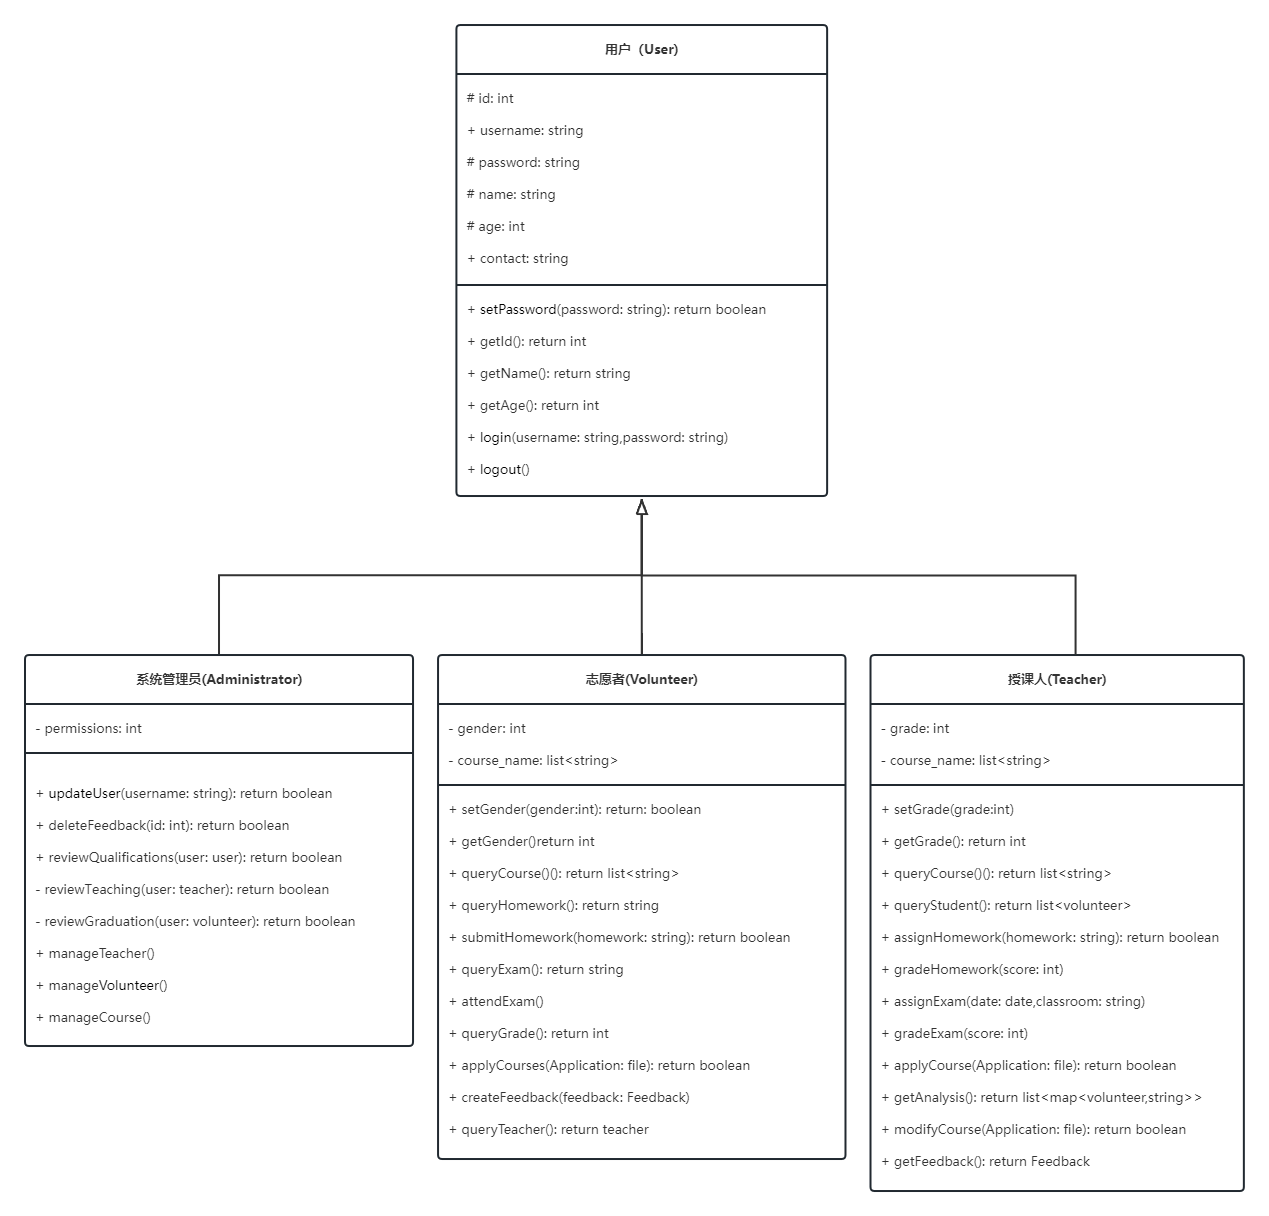
\includegraphics[scale=0.33]{OOA/fig/4-课程管理/课程管理类图 (1).png}} 
    \bicaption{Volunet公益课程系统类属性与操作1子图}{Class Attributes and Operations Sub-Diagram 1 for Course System of Volunet} 
\end{figure}

\begin{figure}[H] 
    \center{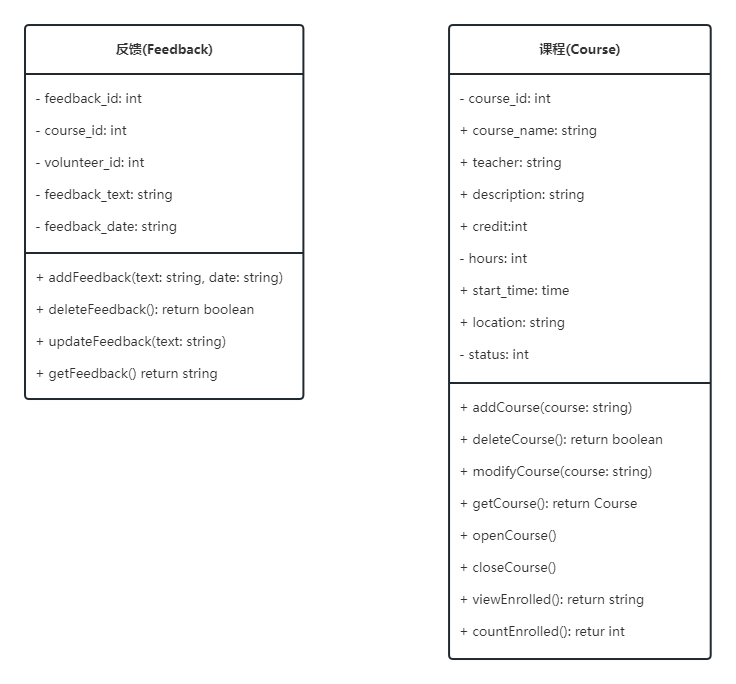
\includegraphics[scale=0.33]{OOA/fig/4-课程管理/课程管理类图 (2).png}} 
    \center{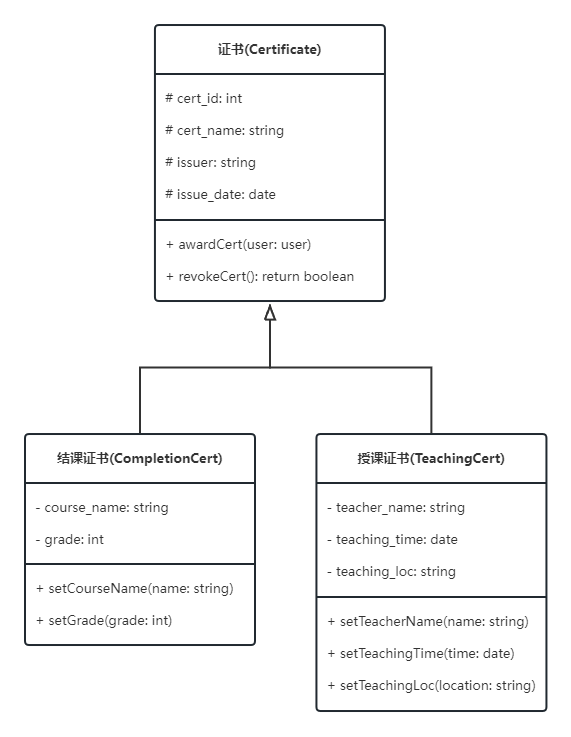
\includegraphics[scale=0.33]{OOA/fig/4-课程管理/课程管理类图 (3).png}} 
    \bicaption{Volunet公益课程系统类属性与操作2子图}{Class Attributes and Operations Sub-Diagram 2 for Course System of Volunet} 
\end{figure}

\begin{figure}[H] 
    \center{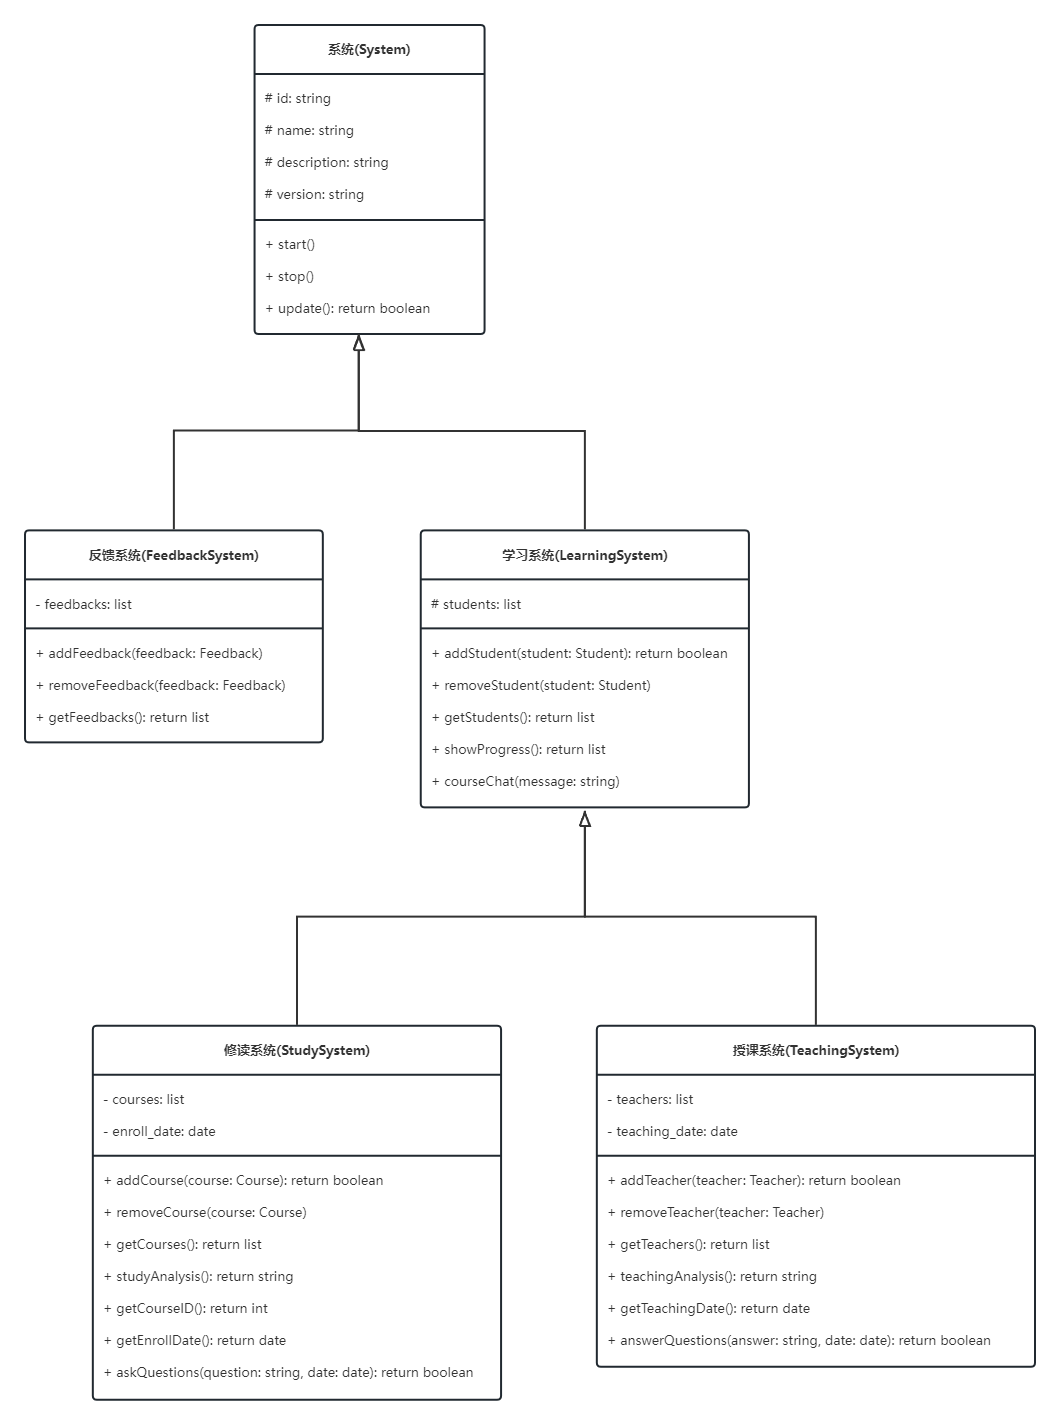
\includegraphics[scale=0.33]{OOA/fig/4-课程管理/课程管理类图 (4).png}} 
    \bicaption{Volunet公益课程系统类属性与操作3子图}{Class Attributes and Operations Sub-Diagram 3 for Course System of Volunet} 
\end{figure}

\paragraph{公益课程系统类属性与操作描述}~{}

公益课程系统中类包含用户、系统管理员、志愿者、授课人、反馈、课程、证书、结课证书、授课证书、系统、反馈系统、学习系统、修读系统、授课系统,它们的属性与操作描述如下:

% 用户、系统管理员、志愿者、授课人、反馈、课程、证书、结课证书、授课证书、系统、反馈系统、学习系统、修读系统、授课系统
\begin{table}[H]  
\caption{“用户”类词条描述}  
\begin{center}  
    \begin{tabular}{l p{11cm}} 
        \hline
        \quad 名称:  &  用户 \\
        \hline
        \quad 编号:  & 4.1 \\
        \hline
        \quad 英文:  &  User \\
        \hline
        \quad 简述:  & 使用课程管理系统的个人的统称 \\
        \hline
        \quad 属性:  & id、username、password、name、age、contact \\
        \hline
        \quad 操作:  & setPassword()、getId()、getName()、getAge() 、login()、logout() \\
        \hline
        \quad 相关类:  & 志愿者、授课人、系统管理员 \\
        \hline
    \end{tabular}
\end{center}
\end{table}


\begin{table}[H]  
\caption{“系统管理员”类词条描述}  
\begin{center}  
    \begin{tabular}{l p{11cm}} 
        \hline
        \quad 名称:  &  系统管理员 \\
        \hline
        \quad 编号:  & 4.2 \\
        \hline
        \quad 英文:  &  Administrator \\
        \hline
        \quad 简述:  & 管理课程信息审核,进行反馈信息审核的人 \\
        \hline
        \quad 属性:  & permissions \\
        \hline
        \quad 操作:  & updateUser()、updateLoveFeedback()、reviewQualifications()、reviewDonation()、reviewOrder()、manageCharitableMerchant()、manageBuyer()、manageTeam()、manageDonor()
\\
        \hline
        \quad 相关类:  & 用户、反馈系统、学习系统 \\
        \hline
    \end{tabular}
\end{center}
\end{table}

\begin{table}[H]  
\caption{“志愿者”类词条描述}  
\begin{center}  
    \begin{tabular}{l p{11cm}} 
        \hline
        \quad 名称:  &  志愿者 \\
        \hline
        \quad 编号:  & 4.3 \\
        \hline
        \quad 英文:  &  Volunteer \\
        \hline
        \quad 简述:  & 使用课程管理系统修读课程,进行课程反馈的人 \\
        \hline
        \quad 属性:  & gender、course\_name \\
        \hline 
        \quad 操作:  & setGender()、getGender()、queryCourse()、queryHomework()、submitHomework()、queryExam()、attendExam()、queryGrade()、applyCourses()、createFeedback()、queryTeacher()\\
        \hline
        \quad 相关类:  & 用户、授课人、修读系统 \\
        \hline
    \end{tabular}
\end{center}
\end{table}

\begin{table}[H]  
\caption{“授课人”类词条描述}  
\begin{center}  
    \begin{tabular}{l p{11cm}} 
        \hline
        \quad 名称:  &  授课人 \\
        \hline
        \quad 编号:  & 4.4 \\
        \hline
        \quad 英文:  &  Teacher \\
        \hline
        \quad 简述:  & 使用课程管理系统对教授课程,回应反馈的人 \\
        \hline
        \quad 属性:  & grade、course\_name \\
        \hline
        \quad 操作:  & setGrade()、getGender()、queryCourse()、queryStudent()、assignHomework()、gradeHomework()、assignExam()、gradeExam()、applyCourse()、getAnalysis()、modifyCourse()、getFeedback() \\
        \hline
        \quad 相关类:  & 用户、志愿者、授课系统 \\
        \hline
    \end{tabular}
\end{center}
\end{table}

\begin{table}[H]  
\caption{“反馈”类词条描述}  
\begin{center}  
    \begin{tabular}{l p{11cm}} 
        \hline
        \quad 名称:  &  反馈 \\
        \hline
        \quad 编号:  & 4.5 \\
        \hline
        \quad 英文:  &  Feedback \\
        \hline
        \quad 简述:  & 志愿者对课程所提交的课程评价 \\
        \hline
        \quad 属性:  & feedback\_id、course\_id、volunteer\_id、feedback\_text、feedback\_date \\
        \hline
        \quad 操作:  & addFeedback()、deleteFeedback()、updateFeedback()、getFeedback()\\
        \hline
        \quad 相关类:  & 反馈系统、修读系统、授课系统 \\
        \hline
    \end{tabular}
\end{center}
\end{table}


\begin{table}[H]  
\caption{“课程”类词条描述}  
\begin{center}  
    \begin{tabular}{l p{11cm}} 
        \hline
        \quad 名称:  &  课程 \\
        \hline
        \quad 编号:  & 4.6 \\
        \hline
        \quad 英文:  &  Course \\
        \hline
        \quad 简述:  & 授课人发布的提高志愿者相关公益技能的项目 \\
        \hline
        \quad 属性:  & course\_id、course\_name、teacher、description、credit、hours、start\_time、location、status \\
        \hline
        \quad 操作:  & addCourse()、deleteCourse()、modifyCourse()、getCourse()、openCourse()、closeCourse()、viewEnrolled()、countEnrolled()\\
        \hline
        \quad 相关类:  & 修读系统、授课系统 \\
        \hline
    \end{tabular}
\end{center}
\end{table}

\begin{table}[H]  
\caption{“证书”类词条描述}  
\begin{center}  
    \begin{tabular}{l p{11cm}} 
        \hline
        \quad 名称:  &  证书 \\
        \hline
        \quad 编号:  & 4.7 \\
        \hline
        \quad 英文:  &  Certificate \\
        \hline
        \quad 简述:  & 对个人或组织具有某种能力、资格或成就的认证文件 \\
        \hline
        \quad 属性:  & cert\_id、cert\_name、issue、issue\_date\\
        \hline
        \quad 操作:  & awardCert()、revokeCert() \\
        \hline
        \quad 相关类:  & 授课证书、结课证书 \\
        \hline
    \end{tabular}
\end{center}
\end{table}

\begin{table}[H]  
\caption{“爱心证书”类词条描述}  
\begin{center}  
    \begin{tabular}{l p{11cm}} 
        \hline
        \quad 名称:  &  爱心证书 \\
        \hline
        \quad 编号:  & 4.8 \\
        \hline
        \quad 英文:  &  CompletionCert \\
        \hline
        \quad 简述:  & 对志愿者学习完课程进行认证的文件 \\
        \hline
        \quad 属性:  & user\_name、grade\\
        \hline
        \quad 操作:  & setCourseName()、setGrade()\\
        \hline
        \quad 相关类:  & 修读系统 \\
        \hline
    \end{tabular}
\end{center}
\end{table}

\begin{table}[H]  
\caption{“授课证书”类词条描述}  
\begin{center}  
    \begin{tabular}{l p{11cm}} 
        \hline
        \quad 名称:  &  授课证书 \\
        \hline
        \quad 编号:  & 4.9 \\
        \hline
        \quad 英文:  &  TeachingCert \\
        \hline
        \quad 简述:  & 对授课人可以教授课程进行认证的文件 \\
        \hline
        \quad 属性:  & teacher\_name、teaching\_time、teaching\_loc\\
        \hline
        \quad 操作:  & setTeacherName()、setTeachingTime()、setTeachingLoc() \\
        \hline
        \quad 相关类:  & 授课系统 \\
        \hline
    \end{tabular}
\end{center}
\end{table}

\begin{table}[H]  
\caption{“系统”类词条描述}  
\begin{center}  
    \begin{tabular}{l p{11cm}} 
        \hline
        \quad 名称:  &  系统 \\
        \hline
        \quad 编号:  & 4.10 \\
        \hline
        \quad 英文:  &  System \\
        \hline
        \quad 简述:  & 课程管理系统的简称 \\
        \hline
        \quad 属性:  & id、name、description、version\\
        \hline
        \quad 操作:  & start()、stop()、update()\\
        \hline
        \quad 相关类:  & 学习系统、反馈系统 \\
        \hline
    \end{tabular}
\end{center}
\end{table}

\begin{table}[H]  
\caption{“反馈系统”类词条描述}  
\begin{center}  
    \begin{tabular}{l p{11cm}} 
        \hline
        \quad 名称:  &  反馈系统 \\
        \hline
        \quad 编号:  & 4.11 \\
        \hline
        \quad 英文:  &  FeedbackSystem \\
        \hline
        \quad 简述:  & 负责对课程进行反馈的系统 \\
        \hline
        \quad 属性:  & feedbacks\\
        \hline
        \quad 操作:  & addFeedback()、removeFeedback()、getFeedbacks()\\
        \hline
        \quad 相关类:  & 系统、系统管理员、反馈 \\
        \hline
    \end{tabular}
\end{center}
\end{table}

\begin{table}[H]  
\caption{“学习系统”类词条描述}  
\begin{center}  
    \begin{tabular}{l p{11cm}} 
        \hline
        \quad 名称:  &  学习系统 \\
        \hline
        \quad 编号:  & 4.12 \\
        \hline
        \quad 英文:  &  LearningSystem \\
        \hline
        \quad 简述:  & 负责教授、学习课程的系统 \\
        \hline
        \quad 属性:  & students\\
        \hline
        \quad 操作:  & addStudent()、removeStudent()、getStudents()、showProgress()、courseChat()
\\
        \hline
        \quad 相关类:  & 系统、系统管理员、修读系统、授课系统 \\
        \hline
    \end{tabular}
\end{center}
\end{table}

\begin{table}[H]  
\caption{“修读系统”类词条描述}  
\begin{center}  
    \begin{tabular}{l p{11cm}} 
        \hline
        \quad 名称:  &  修读系统 \\
        \hline
        \quad 编号:  & 4.13 \\
        \hline
        \quad 英文:  &  StudySystem \\
        \hline
        \quad 简述:  & 负责课程学习、管理学生修读进度的系统 \\
        \hline
        \quad 属性:  & courses、enroll\_date\\
        \hline
        \quad 操作:  & addCourse()、removeCourse()、getCourses()、studyAnalysis()、getCourseID()、getEnrollDate()、askQuestions()\\
        \hline
        \quad 相关类:  & 学习系统、反馈、课程、结课证书、志愿者 \\
        \hline
    \end{tabular}
\end{center}
\end{table}

\begin{table}[H]  
\caption{“授课系统”类词条描述}  
\begin{center}  
    \begin{tabular}{l p{11cm}} 
        \hline
        \quad 名称:  &  授课系统 \\
        \hline
        \quad 编号:  & 4.14 \\
        \hline
        \quad 英文:  &  TeachingSystem \\
        \hline
        \quad 简述:  & 负责教授的课程的管理的系统 \\
        \hline
        \quad 属性:  & teachers、teaching\_date\\
        \hline
        \quad 操作:  & addTeacher()、removeTeacher()、getTeachers()、teachingAnalysis()、getTeachingDate()、answerQuestions()\\
        \hline
        \quad 相关类:  & 学习系统、反馈、课程、授课证书、授课人 \\
        \hline
    \end{tabular}
\end{center}
\end{table}


\subsubsection{交流论坛系统}

\paragraph{交流论坛系统类属性与操作图}~{}
\begin{figure}[H] 
    \center{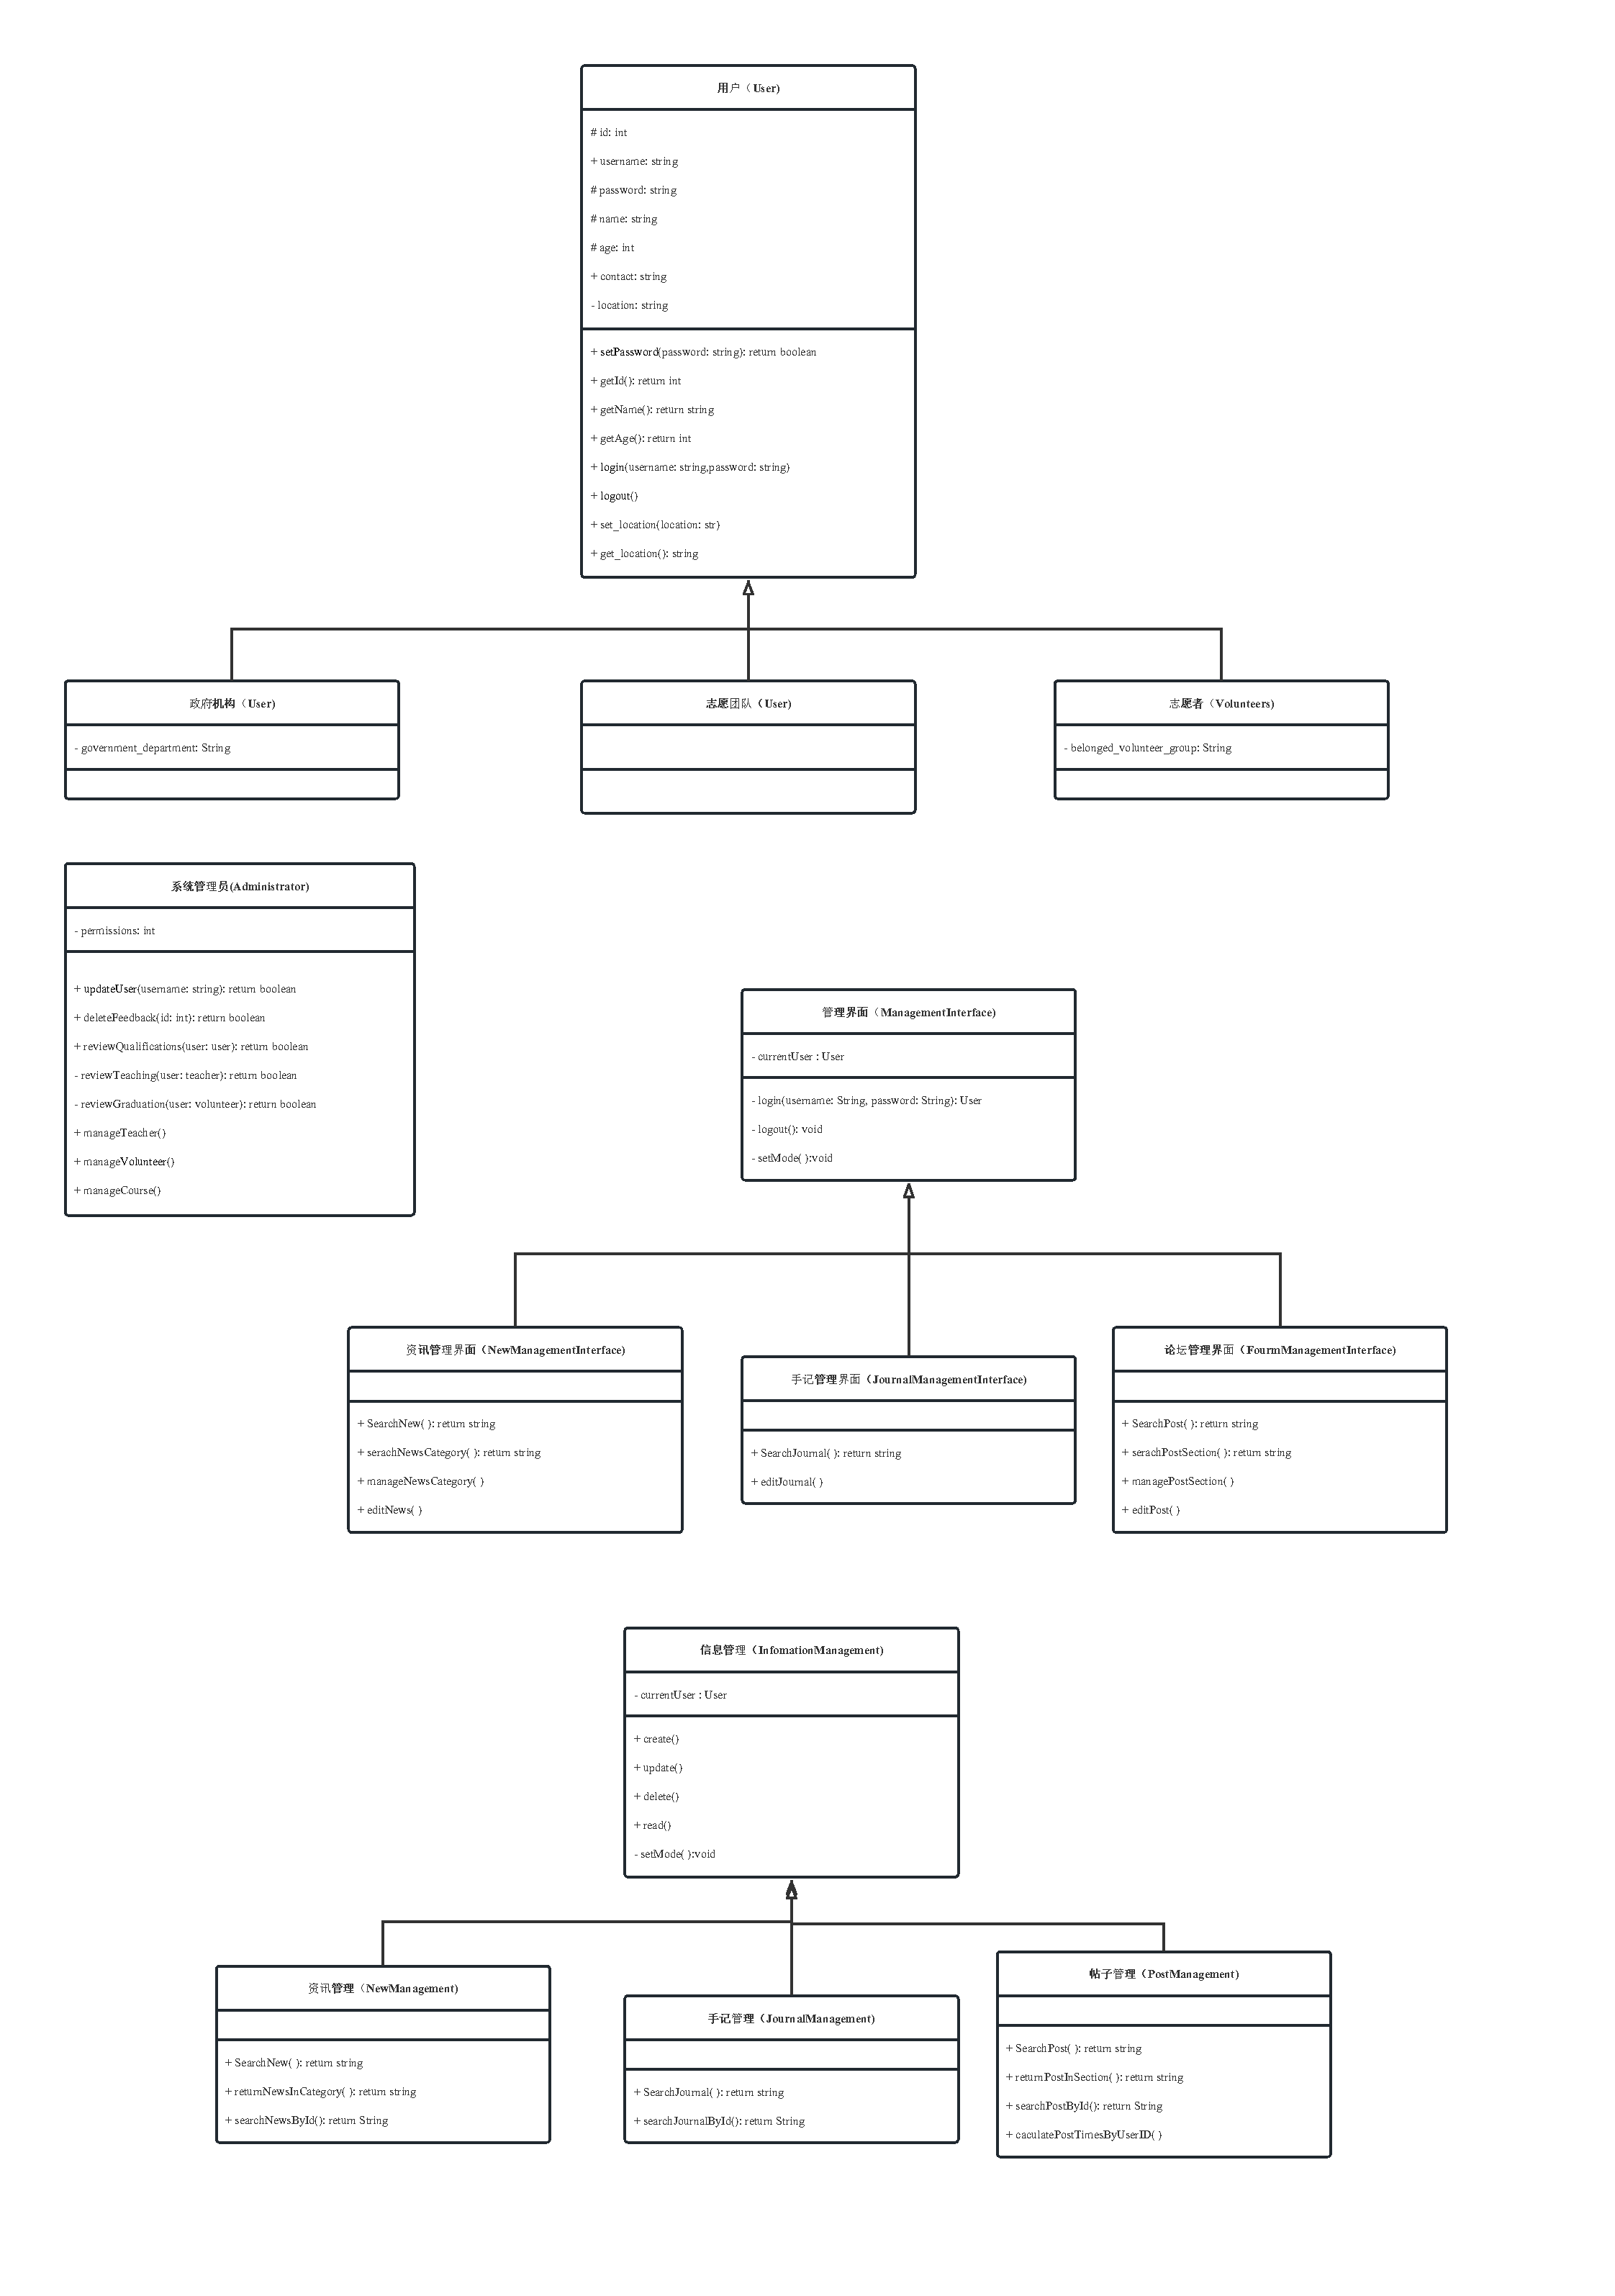
\includegraphics[scale=0.33]{OOA/fig/5-论坛管理/论坛管理类图属性与操作-1.pdf}} 
    \bicaption{Volunet交流论坛系统类属性与操作1子图}{Class Attributes and Operations Sub-Diagram 1 for Communication System of Volunet} 
\end{figure}

% \begin{figure}[H] 
%     \center{\includegraphics[scale=0.33]{OOA/fig/5-论坛管理/论坛管理类图属性与操作-2.pdf}} 
%     \bicaption{Volunet交流论坛系统类属性与操作2子图}{Class Attributes and Operations Sub-Diagram 2 for Communi
%     System of Volunet} 
% \end{figure}

\paragraph{交流论坛系统类属性与操作描述}~{}

交流论坛系统中类包含用户、志愿者、志愿团队、政府结构、管理界面、资讯管理界面、手记管理界面、论坛管理界面、资讯类别管理、资讯管理、资讯评论管理、手记管理、手机评论管理、帖子管理、回帖管理、板块管理、资讯类别、资讯信息、资讯评论、手记信息、手记评论、帖子讯息、板块信息、审计报表生成,它们的属性与操作描述如下:

\begin{table}[H]  
\caption{“系统管理员”类词条描述}  
\begin{center}  
    \begin{tabular}{l p{11cm}} 
        \hline
        \quad 名称:  &  系统管理员 \\
        \hline
        \quad 编号:  & 5.1 \\
        \hline
        \quad 英文:  &  Administrator \\
        \hline
        \quad 简述:  & 交流论坛系统中的管理员 \\
        \hline
        \quad 属性:  & id、username、password、permissions \\
        \hline
        \quad 操作:  & setPassword()、getId()、manageAuditing()、InformationReviewing() \\
        \hline
        \quad 相关类:  & 志愿者、志愿团队、政府机构、管理界面 \\
        \hline
    \end{tabular}
\end{center}
\end{table}

\begin{table}[H]  
\caption{“用户”类词条描述}  
\begin{center}  
    \begin{tabular}{l p{11cm}} 
        \hline
        \quad 名称:  &  用户 \\
        \hline
        \quad 编号:  & 5.2 \\
        \hline
        \quad 英文:  &  User \\
        \hline
        \quad 简述:  & 交流论坛系统中参与的个体的统称 \\
        \hline
        \quad 属性:  & id、username、password、name、age、contact \\
        \hline
        \quad 操作:  & setPassword()、getId()、getName()、getAge() 、login()、logout() \\
        \hline
        \quad 相关类:  & 志愿者、志愿团队、政府机构、管理界面 \\
        \hline
    \end{tabular}
\end{center}
\end{table}

\begin{table}[H]  
\caption{“志愿者”类词条描述}  
\begin{center}  
    \begin{tabular}{l p{11cm}} 
        \hline
        \quad 名称:  &  志愿者 \\
        \hline
        \quad 编号:  & 5.3 \\
        \hline
        \quad 英文:  &  Volunteer \\
        \hline
        \quad 简述:  & 注册登录交流管理系统的个人 \\
        \hline
        \quad 属性:  & id、username、password、name、age、contact、VolunteeringTeam \\
        \hline 
        \quad 操作:  & setPassword()、getId()、getName()、getAge() 、login()、logout()\\
        \hline
        \quad 相关类:  & 用户 \\
        \hline
    \end{tabular}
\end{center}
\end{table}

\begin{table}[H]  
\caption{“志愿团队”类词条描述}  
\begin{center}  
    \begin{tabular}{l p{11cm}} 
        \hline
        \quad 名称:  &  志愿团队 \\
        \hline
        \quad 编号:  & 5.4 \\
        \hline
        \quad 英文:  &  Volunteering Team \\
        \hline
        \quad 简述:  & 注册登录交流管理系统的团体 \\
        \hline
        \quad 属性:  & id、username、password、name、age、contact \\
        \hline
        \quad 操作:  & setPassword()、getId()、getName()、getAge() 、login()、logout() \\
        \hline
        \quad 相关类:  & 用户 \\
        \hline
    \end{tabular}
\end{center}
\end{table}

\begin{table}[H]  
\caption{“政府机构”类词条描述}  
\begin{center}  
    \begin{tabular}{l p{11cm}} 
        \hline
        \quad 名称:  & 政府机构 \\
        \hline
        \quad 编号:  & 5.5 \\
        \hline
        \quad 英文:  &  Government Department \\
        \hline
        \quad 简述:  & 注册登录交流管理系统的政府机构 \\
        \hline
        \quad 属性:  & id、username、password、name、age、contact、departmentName \\
        \hline
        \quad 操作:  & setPassword()、getId()、getName()、getAge() 、login()、logout() \\
        \hline
        \quad 相关类:  & 用户 \\
        \hline
    \end{tabular}
\end{center}
\end{table}

\begin{table}[H]  
\caption{“管理界面”类词条描述}  
\begin{center}  
    \begin{tabular}{l p{11cm}} 
        \hline
        \quad 名称:  & 管理界面 \\
        \hline
        \quad 编号:  & 5.7 \\
        \hline
        \quad 英文:  &  Management Interface \\
        \hline
        \quad 简述:  & 用户管理交流信息的界面 \\
        \hline
        \quad 属性:  & currentUser \\
        \hline
        \quad 操作:  & login()、logout()、setMode() \\
        \hline
        \quad 相关类: & 用户、资讯管理界面、手记管理界面、论坛管理界面\\
        \hline
    \end{tabular}
\end{center}
\end{table}

%资讯管理

\begin{table}[H]  
\caption{“资讯管理界面”类词条描述}  
\begin{center}  
    \begin{tabular}{l p{11cm}} 
        \hline
        \quad 名称:  & 资讯管理界面 \\
        \hline
        \quad 编号:  & 5.8 \\
        \hline
        \quad 英文:  &  News Management Interface \\
        \hline
        \quad 简述:  & 用户管理资讯的界面 \\
        \hline
        \quad 属性:  & currentUser \\
        \hline
        \quad 操作:  & login()、logout()、SearchNew()、serachNewsCategory()、manageNewsCategory()、editNews( )\\
        \hline
        \quad 相关类: & 管理界面、资讯类别管理、资讯管理、资讯评论管理\\
        \hline
    \end{tabular}
\end{center}
\end{table}

\begin{table}[H]  
\caption{“资讯类别管理”类词条描述}  
\begin{center}  
    \begin{tabular}{l p{11cm}} 
        \hline
        \quad 名称:  & 资讯类别管理 \\
        \hline
        \quad 编号:  & 5.9 \\
        \hline
        \quad 英文:  &  News Category Management\\
        \hline
        \quad 简述:  & 用户管理资讯类别的系统 \\
        \hline
        \quad 属性:  & currentUser \\
        \hline
        \quad 操作:  & addNewsCategory( )、deleteNewsCategory()、searchNewCategory( )\\
        \hline
        \quad 相关类: & 资讯管理界面、资讯类别\\
        \hline
    \end{tabular}
\end{center}
\end{table}

\begin{table}[H]  
\caption{“资讯管理”类词条描述}  
\begin{center}  
    \begin{tabular}{l p{11cm}} 
        \hline
        \quad 名称:  & 资讯管理 \\
        \hline
        \quad 编号:  & 5.10 \\
        \hline
        \quad 英文:  &  News Management\\
        \hline
        \quad 简述:  & 用户管理资讯信息的系统 \\
        \hline
        \quad 属性:  & currentUser \\
        \hline
        \quad 操作:  & SearchNews( )、returnNewsInCategory( )、searchNewsById()\\
        \hline
        \quad 相关类: & 资讯管理界面、资讯类别、资讯信息、资讯评论\\
        \hline
    \end{tabular}
\end{center}
\end{table}

\begin{table}[H]  
\caption{“资讯评论管理”类词条描述}  
\begin{center}  
    \begin{tabular}{l p{11cm}} 
        \hline
        \quad 名称:  & 资讯评论管理 \\
        \hline
        \quad 编号:  & 5.11 \\
        \hline
        \quad 英文:  &  News Comment Management\\
        \hline
        \quad 简述:  & 用户管理资讯所属评论的系统 \\
        \hline
        \quad 属性:  & currentUser \\
        \hline
        \quad 操作:  & SearchNewsComment( ) \\
        \hline
        \quad 相关类: & 资讯管理界面、资讯评论\\
        \hline
    \end{tabular}
\end{center}
\end{table}

\begin{table}[H]  
\caption{“资讯类型”类词条描述}  
\begin{center}  
    \begin{tabular}{l p{11cm}} 
        \hline
        \quad 名称:  & 资讯类型 \\
        \hline
        \quad 编号:  & 5.12 \\
        \hline
        \quad 英文:  &  News Category\\
        \hline
        \quad 简述:  & 资讯的类型 \\
        \hline
        \quad 属性:  & currentUser \\
        \hline
        \quad 操作:  & SearchNew( )、returnNewsInCategory( )、searchNewsById()\\
        \hline
        \quad 相关类: & 资讯管理、资讯类型管理、资讯信息\\
        \hline
    \end{tabular}
\end{center}
\end{table}

\begin{table}[H]  
\caption{“资讯信息”类词条描述}  
\begin{center}  
    \begin{tabular}{l p{11cm}} 
        \hline
        \quad 名称:  & 资讯信息 \\
        \hline
        \quad 编号:  & 5.13 \\
        \hline
        \quad 英文:  &  News Information\\
        \hline
        \quad 简述:  & 资讯的信息 \\
        \hline
        \quad 属性:  & newsID、newsName、newsContent、newsLength、newsAuthor \\
        \hline
        \quad 操作:  & addNews( )、editNews( )\\
        \hline
        \quad 相关类: & 资讯管理、资讯类别、资讯评论、审计报表生成\\
        \hline
    \end{tabular}
\end{center}
\end{table}

\begin{table}[H]  
\caption{“资讯评论”类词条描述}  
\begin{center}  
    \begin{tabular}{l p{11cm}} 
        \hline
        \quad 名称:  & 资讯评论 \\
        \hline
        \quad 编号:  & 5.14 \\
        \hline
        \quad 英文:  &  News Comment\\
        \hline
        \quad 简述:  & 资讯的评论 \\
        \hline
        \quad 属性:  & newsCommentID、newsCommentContent、newsCommentLength、newsCommentAuthor\\
        \hline
        \quad 操作:  & addNewsComment( )、ModifyNewsComment( )、DeleteNewsComment( )、SearchNewsComment( ) \\
        \hline
        \quad 相关类: & 资讯管理、资讯评论管理、资讯信息\\
        \hline
    \end{tabular}
\end{center}
\end{table}

%手记管理

\begin{table}[H]  
\caption{“手记管理界面”类词条描述}  
\begin{center}  
    \begin{tabular}{l p{11cm}} 
        \hline
        \quad 名称:  & 手记管理界面 \\
        \hline
        \quad 编号:  & 5.15 \\
        \hline
        \quad 英文:  &  Journal Management Interface \\
        \hline
        \quad 简述:  & 用户管理资讯的界面 \\
        \hline
        \quad 属性:  & currentUser \\
        \hline
        \quad 操作:  & login()、logout()、SearchJournal()、editJournal( )\\
        \hline
        \quad 相关类: & 管理界面、手记管理、手记评论管理\\
        \hline
    \end{tabular}
\end{center}
\end{table}

\begin{table}[H]  
\caption{“手记管理”类词条描述}  
\begin{center}  
    \begin{tabular}{l p{11cm}} 
        \hline
        \quad 名称:  & 手记管理 \\
        \hline
        \quad 编号:  & 5.16 \\
        \hline
        \quad 英文:  &  Journal Management\\
        \hline
        \quad 简述:  & 用户管理手记信息的系统 \\
        \hline
        \quad 属性:  & currentUser \\
        \hline
        \quad 操作:  & SearchJournal( )、searchJournalById()\\
        \hline
        \quad 相关类: & 手记管理界面、手记信息、手记评论\\
        \hline
    \end{tabular}
\end{center}
\end{table}

\begin{table}[H]  
\caption{“手记评论管理”类词条描述}  
\begin{center}  
    \begin{tabular}{l p{11cm}} 
        \hline
        \quad 名称:  & 手记评论管理 \\
        \hline
        \quad 编号:  & 5.17 \\
        \hline
        \quad 英文:  &  Journal Comment Management\\
        \hline
        \quad 简述:  & 用户管理手记所属评论的系统 \\
        \hline
        \quad 属性:  & currentUser \\
        \hline
        \quad 操作:  & SearchjournalComment( ) \\
        \hline
        \quad 相关类: & 手记管理界面、手记评论\\
        \hline
    \end{tabular}
\end{center}
\end{table}

\begin{table}[H]  
\caption{“手记信息”类词条描述}  
\begin{center}  
    \begin{tabular}{l p{11cm}} 
        \hline
        \quad 名称:  & 手记信息 \\
        \hline
        \quad 编号:  & 5.18 \\
        \hline
        \quad 英文:  &  Journal Information\\
        \hline
        \quad 简述:  & 手记的信息 \\
        \hline
        \quad 属性:  & journalID、journalName、journalContent、journalLength、journalAuthor \\
        \hline
        \quad 操作:  & addJournal( )、editJournal( )\\
        \hline
        \quad 相关类: & 手记管理、手记评论、审计报表生成\\
        \hline
    \end{tabular}
\end{center}
\end{table}

\begin{table}[H]  
\caption{“手记评论”类词条描述}  
\begin{center}  
    \begin{tabular}{l p{11cm}} 
        \hline
        \quad 名称:  & 手记评论 \\
        \hline
        \quad 编号:  & 5.19 \\
        \hline
        \quad 英文:  &  journal Comment\\
        \hline
        \quad 简述:  & 手记的评论 \\
        \hline
        \quad 属性:  & journalCommentID、journalCommentContent、journalCommentLength、journalCommentAuthor\\
        \hline
        \quad 操作:  & addJournalComment( )、ModifyJournalComment( )、DeleteJournalComment( )、SearchJournalComment( ) \\
        \hline
        \quad 相关类: & 手记管理、手记评论管理、手记信息\\
        \hline
    \end{tabular}
\end{center}
\end{table}

%论坛管理

\begin{table}[H]  
\caption{“论坛管理界面”类词条描述}  
\begin{center}  
    \begin{tabular}{l p{11cm}} 
        \hline
        \quad 名称:  & 论坛管理界面 \\
        \hline
        \quad 编号:  & 5.20 \\
        \hline
        \quad 英文:  &  Fourm Management Interface \\
        \hline
        \quad 简述:  & 用户管理论坛的界面 \\
        \hline
        \quad 属性:  & currentUser \\
        \hline
        \quad 操作:  & login()、logout()、SearchPost( )、erachPostSection( )、managePostSection( )、editPost( )\\
        \hline
        \quad 相关类: & 管理界面、论坛板块管理、帖子管理、板块管理\\
        \hline
    \end{tabular}
\end{center}
\end{table}

\begin{table}[H]  
\caption{“板块管理”类词条描述}  
\begin{center}  
    \begin{tabular}{l p{11cm}} 
        \hline
        \quad 名称:  & 板块管理 \\
        \hline
        \quad 编号:  & 5.21 \\
        \hline
        \quad 英文:  &  Fourm Section Management\\
        \hline
        \quad 简述:  & 用户管理论坛板块的系统 \\
        \hline
        \quad 属性:  & currentUser \\
        \hline
        \quad 操作:  & addFourmSection( )、ModifyFourmSection( )、DeleteFourmSection( )、SearchFourmSection( )\\
        \hline
        \quad 相关类: & 论坛管理界面、论坛板块\\
        \hline
    \end{tabular}
\end{center}
\end{table}

\begin{table}[H]  
\caption{“帖子管理”类词条描述}  
\begin{center}  
    \begin{tabular}{l p{11cm}} 
        \hline
        \quad 名称:  & 帖子管理 \\
        \hline
        \quad 编号:  & 5.22 \\
        \hline
        \quad 英文:  &  Post Management\\
        \hline
        \quad 简述:  & 用户管理帖子信息的系统 \\
        \hline
        \quad 属性:  & currentUser \\
        \hline
        \quad 操作:  & SearchPost( )、returnPostInSection( )、searchPostById()、caculatePostTimesByUserID( )\\
        \hline
        \quad 相关类: & 论坛管理界面、帖子信息、板块信息\\
        \hline
    \end{tabular}
\end{center}
\end{table}

\begin{table}[H]  
\caption{“回帖管理”类词条描述}  
\begin{center}  
    \begin{tabular}{l p{11cm}} 
        \hline
        \quad 名称:  & 资讯评论管理 \\
        \hline
        \quad 编号:  & 5.23 \\
        \hline
        \quad 英文:  &  Post Respond Management\\
        \hline
        \quad 简述:  & 用户管理资讯所属评论的系统 \\
        \hline
        \quad 属性:  & currentUser \\
        \hline
        \quad 操作:  & SearchPostRespondList( )、caculateRespondTimesByUserID( )、caculatePostNumberBySection( ) \\
        \hline
        \quad 相关类: & 论坛管理界面、帖子信息\\
        \hline
    \end{tabular}
\end{center}
\end{table}

\begin{table}[H]  
\caption{“板块信息”类词条描述}  
\begin{center}  
    \begin{tabular}{l p{11cm}} 
        \hline
        \quad 名称:  & 板块信息 \\
        \hline
        \quad 编号:  & 5.24 \\
        \hline
        \quad 英文:  &  Section Information\\
        \hline
        \quad 简述:  & 论坛板块的信息 \\
        \hline
        \quad 属性:  & sectionID\\
        \hline
        \quad 操作:  & modifySection()\\
        \hline
        \quad 相关类: & 板块管理、帖子管理、帖子信息\\
        \hline
    \end{tabular}
\end{center}
\end{table}

\begin{table}[H]  
\caption{“帖子信息”类词条描述}  
\begin{center}  
    \begin{tabular}{l p{11cm}} 
        \hline
        \quad 名称:  & 帖子信息 \\
        \hline
        \quad 编号:  & 5.25 \\
        \hline
        \quad 英文:  &  Post Information\\
        \hline
        \quad 简述:  & 帖子的信息 \\
        \hline
        \quad 属性:  & PostID、PostName、PostContent、PostLength、PostAuthor、PostSection \\
        \hline
        \quad 操作:  & addPost( )、editPost( )\\
        \hline
        \quad 相关类: & 帖子管理、回帖管理、板块信息、审计报表生成\\
        \hline
    \end{tabular}
\end{center}
\end{table}

%审计报表生成

\begin{table}[H]  
\caption{“审计报表”类词条描述}  
\begin{center}  
    \begin{tabular}{l p{11cm}} 
        \hline
        \quad 名称:  & 审计报表 \\
        \hline
        \quad 编号:  & 5.26 \\
        \hline
        \quad 英文:  &  Audit Report\\
        \hline
        \quad 简述:  & 根据系统信息生成的审计报表 \\
        \hline
        \quad 属性:  & currentUser \\
        \hline
        \quad 操作:  & GenerateByTime()、GetAuditionRepoet()\\
        \hline
        \quad 相关类: & 资讯信息、手记信息、帖子信息、系统管理员\\
        \hline
    \end{tabular}
\end{center}
\end{table}


\subsubsection{志愿交友系统}

\paragraph{志愿交友系统类属性与操作图}~{}
\begin{figure}[H] 
    \center{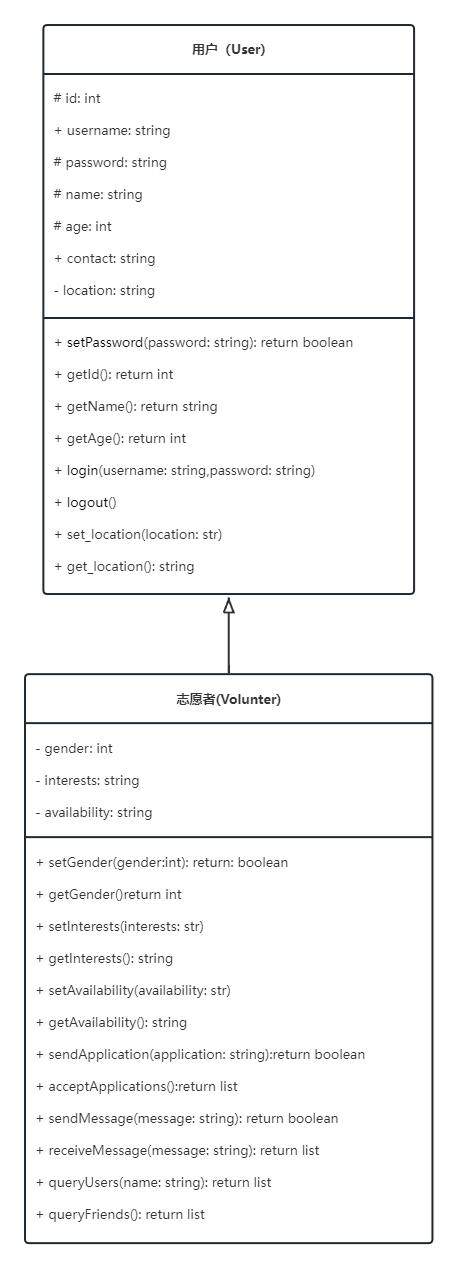
\includegraphics[scale=0.3]{OOA/fig/6-交友管理/志愿交友管理类图 (1).png}} 
    \bicaption{Volunet志愿交友系统类属性与操作1子图}{Class Attributes and Operations Sub-Diagram 1 for Volunteer Friends System of Volunet} 
\end{figure}

\begin{figure}[H] 
    \center{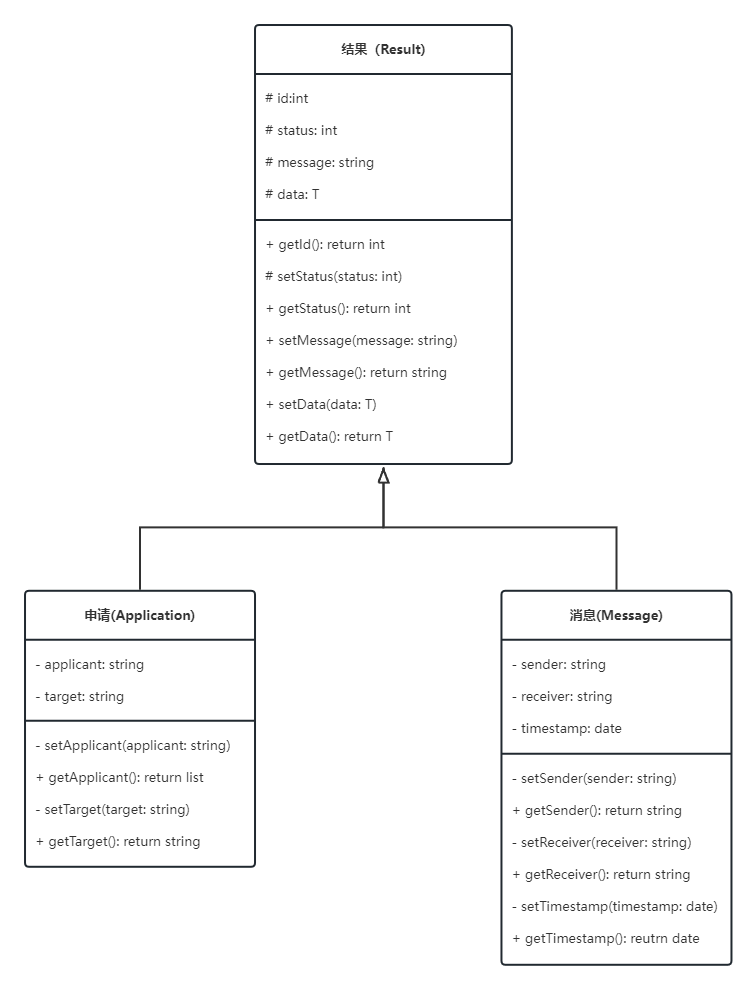
\includegraphics[scale=0.3]{OOA/fig/6-交友管理/志愿交友管理类图 (2).png}} 
    \center{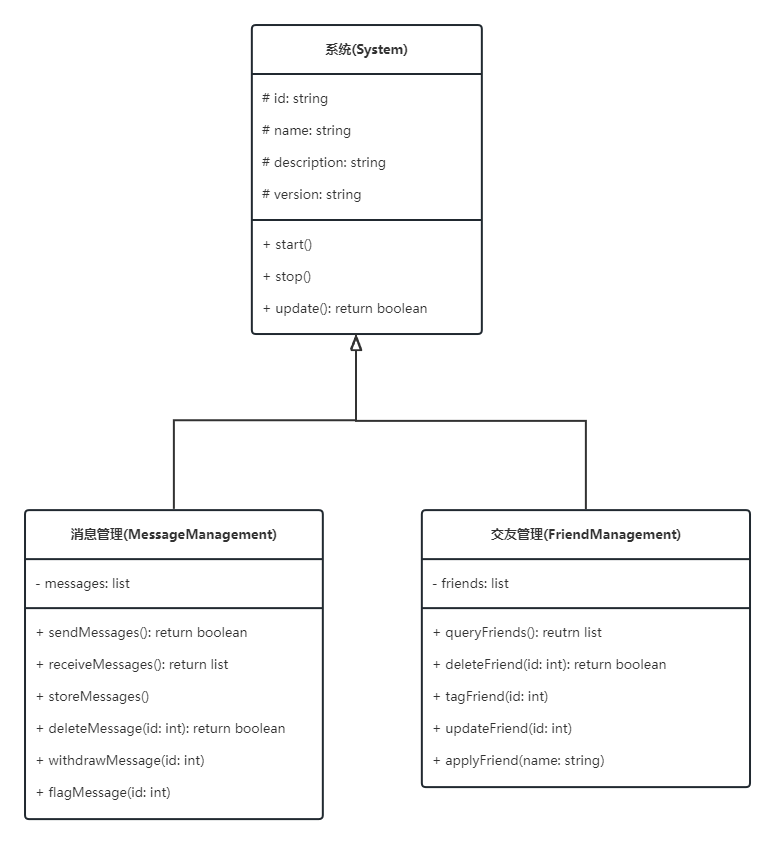
\includegraphics[scale=0.35]{OOA/fig/6-交友管理/志愿交友管理类图 (3).png}} 
    \bicaption{Volunet志愿交友系统类属性与操作2子图}{Class Attributes and Operations Sub-Diagram 2 for Volunteer Friends System of Volunet} 
\end{figure}

\paragraph{志愿交友系统类属性与操作描述}~{}

爱心捐助系统中类包含用户、志愿者、结果、申请、反馈、系统、消息管理、交友管理,它们的属性与操作描述如下:

% 用户、志愿者、结果、消息、申请、系统、交友管理系统、消息管理系统
\begin{table}[H]  
\caption{“用户”类词条描述}  
\begin{center}  
    \begin{tabular}{l p{11cm}} 
        \hline
        \quad 名称:  &  用户 \\
        \hline
        \quad 编号:  & 6.1 \\
        \hline
        \quad 英文:  &  User \\
        \hline
        \quad 简述:  & 使用交友管理系统和消息管理系统的个人的统称 \\
        \hline
        \quad 属性:  & id、username、password、name、age、contact \\
        \hline
        \quad 操作:  & setPassword()、getId()、getName()、getAge() 、login()、logout() \\
        \hline
        \quad 相关类:  & 志愿者 \\
        \hline
    \end{tabular}
\end{center}
\end{table}

\begin{table}[H]  
\caption{“志愿者”类词条描述}  
\begin{center}  
    \begin{tabular}{l p{11cm}} 
        \hline
        \quad 名称:  &  志愿者 \\
        \hline
        \quad 编号:  & 6.2 \\
        \hline
        \quad 英文:  &  Volunteer \\
        \hline
        \quad 简述:  & 使用交友管理系统和消息管理系统的个人 \\
        \hline
        \quad 属性:  & gender、interests、availability \\
        \hline 
        \quad 操作:  & setInterests()、getInterests()、setAvailability()、getAvailability()、sendApplication()、acceptApplications()、sendMessage()、receiveMessage()、queryUsers()、queryFriends()\\
        \hline
        \quad 相关类:  & 用户、交友管理系统、消息管理系统 \\
        \hline
    \end{tabular}
\end{center}
\end{table}


\begin{table}[H]  
\caption{“结果”类词条描述}  
\begin{center}  
    \begin{tabular}{l p{11cm}} 
        \hline
        \quad 名称:  &  结果 \\
        \hline
        \quad 编号:  & 6.3 \\
        \hline
        \quad 英文:  &  Result \\
        \hline
        \quad 简述:  & 完成交友管理、消息管理后所产生的输出、效果或影响 \\
        \hline
        \quad 属性:  & id、status、message、data\\
        \hline
        \quad 操作:  & getId()、setStatus()、getStatus()、setMessage()、getMessage()、setData()、getData() \\
        \hline
        \quad 相关类:  & 消息、申请 \\
        \hline
    \end{tabular}
\end{center}
\end{table}

\begin{table}[H]  
\caption{“消息”类词条描述}  
\begin{center}  
    \begin{tabular}{l p{11cm}} 
        \hline
        \quad 名称:  &  消息 \\
        \hline
        \quad 编号:  & 6.4 \\
        \hline
        \quad 英文:  &  Message \\
        \hline
        \quad 简述:  & 好友之间相互发送的文本、图像、视频信息 \\
        \hline
        \quad 属性:  & sender、receiver、timestamp \\
        \hline
        \quad 操作:  & setSender()、getSender()、setReceiver()、getReceiver()、setTimestamp()、getTimestamp()\\
        \hline
        \quad 相关类:  & 消息管理、志愿者、结果\\
        \hline
    \end{tabular}
\end{center}
\end{table}



\begin{table}[H]  
\caption{“申请”类词条描述}  
\begin{center}  
    \begin{tabular}{l p{11cm}} 
        \hline
        \quad 名称:  &  申请 \\
        \hline
        \quad 编号:  & 6.5 \\
        \hline
        \quad 英文:  &  Application \\
        \hline
        \quad 简述:  & 队其他用户请求添加好友的文件 \\
        \hline
        \quad 属性:  & applicant、target\\
        \hline
        \quad 操作:  & setApplicant()、getApplicant()、setTarget()、getTarget()\\
        \hline
        \quad 相关类:  & 志愿者、结果、交友管理 \\
        \hline
    \end{tabular}
\end{center}
\end{table}

\begin{table}[H]  
\caption{“系统”类词条描述}  
\begin{center}  
    \begin{tabular}{l p{11cm}} 
        \hline
        \quad 名称:  &  系统 \\
        \hline
        \quad 编号:  & 6.6 \\
        \hline
        \quad 英文:  &  System \\
        \hline
        \quad 简述:  & 进行管理的系统的统称 \\
        \hline
        \quad 属性:  & id、name、description、version\\
        \hline
        \quad 操作:  & start()、stop()、update()\\
        \hline
        \quad 相关类:  & 消息管理系统、交友管理系统 \\
        \hline
    \end{tabular}
\end{center}
\end{table}

\begin{table}[H]  
\caption{“交友管理系统”类词条描述}  
\begin{center}  
    \begin{tabular}{l p{11cm}} 
        \hline
        \quad 名称:  &  交友管理系统 \\
        \hline
        \quad 编号:  & 6.7 \\
        \hline
        \quad 英文:  &  FriendManagementSystem \\
        \hline
        \quad 简述:  & 负责对交友申请和用户好友进行管理和处理的系统 \\
        \hline
        \quad 属性:  & friends\\
        \hline
        \quad 操作:  & queryFriends()、deleteFriend()、tagFriend()、updateFriend()、applyFriend()\\
        \hline
        \quad 相关类:  & 系统、申请 \\
        \hline
    \end{tabular}
\end{center}
\end{table}

\begin{table}[H]  
\caption{“消息管理系统”类词条描述}  
\begin{center}  
    \begin{tabular}{l p{11cm}} 
        \hline
        \quad 名称:  &  消息管理系统 \\
        \hline
        \quad 编号:  & 6.8 \\
        \hline
        \quad 英文:  &  MessageManagementSystem \\
        \hline
        \quad 简述:  & 负责管理用户聊天消息和用户之间的消息记录的系统 \\
        \hline
        \quad 属性:  & messages\\
        \hline
        \quad 操作:  & sendMessages()、receiveMessages()、storeMessages()、deleteMessage()、withdrawMessage()、flagMessage()\\
        \hline
        \quad 相关类:  & 系统、消息 \\
        \hline
    \end{tabular}
\end{center}
\end{table}



% \subsection{交互设计}



\newpage
